% Problems, Chapter 6: Maxwell Equations, Macroscopic Electromagnetism, Conservation Laws
% Jackson, Classical Electrodynamics, 3rd ed.
% Requires: amsmath, amssymb, tikz

\section*{Problems}

\Needspace{5\baselineskip}
\par\bigskip
\noindent\textbf{6.1}\quad In three dimensions the solution to the wave equation (6.32) for a point source in space and time (a light flash at $t'=0$, $\mathbf{x}'=0$) is a spherical shell disturbance of radius $R=ct$, namely the Green function $G^{(+)}$ (6.44). It may be initially surprising that in one or two dimensions, the disturbance possesses a ``wake,'' even though the source is a ``point'' in space and time. The solutions for fewer dimensions than three can be found by superposition in the superfluous dimension(s), to eliminate dependence on such variable(s). For example, a flashing line source of uniform amplitude is equivalent to a point source in two dimensions.
\begin{enumerate}
\item[(a)] Starting with the retarded solution to the three-dimensional wave equation (6.47), show that the source $f(\mathbf{x}',t')=\delta(x')\delta(y')\delta(t')$, equivalent to a $t=0$ point source at the origin in two spatial dimensions, produces a two-dimensional wave,
\[
\Psi(x,y,t)=\frac{2c\Theta(ct-\rho)}{\sqrt{c^{2}t^{2}-\rho^{2}}}
\]
where $\rho^{2}=x^{2}+y^{2}$ and $\Theta(\xi)$ is the unit step function [$\Theta(\xi)=0$ ($1$) if $\xi<0$ ($>0$).]
\item[(b)] Show that a ``sheet'' source, equivalent to a point pulsed source at the origin in one space dimension, produces a one-dimensional wave proportional to
\[
\Psi(x,t)=2\pi c\,\Theta(ct-|x|)
\]
\end{enumerate}
\solution

The normalization in (6.32) is $(\nabla^2-c^{-2}\partial_t^2)\Psi=-4\pi f$;
thus (6.47), with no incident homogeneous wave, gives
\[
\Psi(\mathbf x,t)=\int\frac{f(\mathbf x',t-|\mathbf x-\mathbf x'|/c)}
{|\mathbf x-\mathbf x'|}\,d^3x'.
\]
\textbf{(a)} Translation invariance along $z$ permits setting the observation
point's $z$ coordinate to zero. Put $R=(\rho^2+z'^2)^{1/2}$. Then
\[
\Psi=\int_{-\infty}^{\infty}\frac{\delta(t-R/c)}R\,dz'.
\]
There are no roots for $ct<\rho$. For $ct>\rho$ the two roots are
$z'_\pm=\pm\sqrt{c^2t^2-\rho^2}$, and
$|d(t-R/c)/dz'|=|z'|/(cR)$. Hence each root contributes
$c/\sqrt{c^2t^2-\rho^2}$, proving
\[
\boxed{\Psi=\frac{2c\Theta(ct-\rho)}{\sqrt{c^2t^2-\rho^2}}.}
\]
The inverse square root at the wavefront is understood as a locally
integrable distribution, not as a finite pointwise value on the front.

\textbf{(b)} For $f=\delta(x')\delta(t')$, use polar coordinates $s,\varphi$
in the source $y'z'$ plane and $R=(x^2+s^2)^{1/2}$:
\[
\Psi=2\pi\int_0^\infty\frac{s\,ds}{\sqrt{x^2+s^2}}
\delta\left(t-\frac{\sqrt{x^2+s^2}}c\right)
=2\pi\int_{|x|}^{\infty}\delta(t-R/c)\,dR
=\boxed{2\pi c\Theta(ct-|x|)}.
\]
For a fixed observation point, progressively more distant portions of the
line or sheet contribute after the earliest arrival. Their superposition
explains the wake without introducing a propagation speed other than $c$.

\Needspace{5\baselineskip}
\par\bigskip
\noindent\textbf{6.2}\quad The charge and current densities for a single point charge $q$ can be written formally as
\[
\rho(\mathbf{x}',t')=q\delta[\mathbf{x}'-\mathbf{r}(t')];\qquad \mathbf{J}(\mathbf{x}',t')=q\mathbf{v}(t')\delta[\mathbf{x}'-\mathbf{r}(t')]
\]
where $\mathbf{r}(t')$ is the charge's position at time $t'$ and $\mathbf{v}(t')$ is its velocity. In evaluating expressions involving the retarded time, one must put $t'=t_{\mathrm{ret}}=t-R(t')/c$, where $\mathbf{R}=\mathbf{x}-\mathbf{r}(t')$ (but $\mathbf{R}=\mathbf{x}-\mathbf{x}'$ ($t'$) inside the delta functions).
\erratum{Assume a smooth subluminal trajectory and an observation event off
the worldline with a finite retarded intersection. Subluminal motion alone
ensures uniqueness, but does not ensure that such an intersection exists.}
\begin{enumerate}
\item[(a)] As a preliminary to deriving the Heaviside--Feynman expressions for the electric and magnetic fields of a point charge, show that
\[
\int d^{3}x'\;\delta[\mathbf{x}'-\mathbf{r}(t_{\mathrm{ret}})]=\frac{1}{\kappa}
\]
where $\kappa=1-\mathbf{v}\cdot\hat{\mathbf{R}}/c$. Note that $\kappa$ is evaluated at the retarded time.
\item[(b)] Starting with the Jefimenko generalizations of the Coulomb and Biot--Savart laws, use the expressions for the charge and current densities for a point charge and the result of part a to obtain the Heaviside--Feynman expressions for the electric and magnetic fields of a point charge,
\[
\mathbf{E}=\frac{q}{4\pi\epsilon_{0}}\left\{\left[\frac{\hat{\mathbf{R}}}{\kappa R^{2}}\right]_{\mathrm{ret}}+\frac{\partial}{c\partial t}\left[\frac{\hat{\mathbf{R}}}{\kappa R}\right]_{\mathrm{ret}}-\frac{\partial}{c^{2}\partial t}\left[\frac{\mathbf{v}}{\kappa R}\right]_{\mathrm{ret}}\right\}
\]
and
\[
\mathbf{B}=\frac{\mu_{0}q}{4\pi}\left\{\left[\frac{\mathbf{v}\times\hat{\mathbf{R}}}{\kappa R^{2}}\right]_{\mathrm{ret}}+\frac{\partial}{c\partial t}\left[\frac{\mathbf{v}\times\hat{\mathbf{R}}}{\kappa R}\right]_{\mathrm{ret}}\right\}
\]
\item[(c)] In our notation Feynman's expression for the electric field is
\[
\mathbf{E}=\frac{q}{4\pi\epsilon_{0}}\left\{\left[\frac{\hat{\mathbf{R}}}{R^{2}}\right]_{\mathrm{ret}}+\frac{[R]_{\mathrm{ret}}}{c}\frac{\partial}{\partial t}\left[\frac{\hat{\mathbf{R}}}{R^{2}}\right]_{\mathrm{ret}}+\frac{\partial^{2}}{c^{2}\partial t^{2}}\left[\hat{\mathbf{R}}\right]_{\mathrm{ret}}\right\}
\]
while Heaviside's expression for the magnetic field is
\[
\mathbf{B}=\frac{\mu_{0}q}{4\pi}\left\{\left[\frac{\mathbf{v}\times\hat{\mathbf{R}}}{\kappa^{2}R^{2}}\right]_{\mathrm{ret}}+\frac{1}{c[R]_{\mathrm{ret}}}\frac{\partial}{\partial t}\left[\frac{\mathbf{v}\times\hat{\mathbf{R}}}{\kappa}\right]_{\mathrm{ret}}\right\}
\]
Show the equivalence of the two sets of expressions for the fields.
\end{enumerate}
\emph{References}: O. Heaviside, \emph{Electromagnetic Theory}, Vol.~3 (1912), p.~464, Eq.~(214). R.~P. Feynman, \emph{The Feynman Lectures in Physics}, Vol.~1 (1963), Chapter 28, Eq. (28.3).
\solution

Assume a smooth subluminal trajectory and an observation event off the
worldline whose past light cone intersects the trajectory at a finite time.
Write $s=t_{\rm ret}$, $\mathbf n=\hat{\mathbf R}$, $v_n=\mathbf v\cdot\mathbf n$,
and $\kappa=1-v_n/c>0$. Quantities below are evaluated at $s$ unless stated otherwise.

\textbf{(a)} In the spatial integral the retarded time is
$s(\mathbf x')=t-|\mathbf x-\mathbf x'|/c$, so
$\partial s/\partial x'_j=n_j/c$. The derivative matrix of the delta
function's argument is
\[
\frac{\partial[x'_i-r_i(s(\mathbf x'))]}{\partial x'_j}
=\delta_{ij}-\frac{v_i n_j}{c},\qquad
\det\left(\mathbf1-\frac{\mathbf v\mathbf n^{\mathsf T}}c\right)
=1-\frac{\mathbf n\cdot\mathbf v}c=\kappa.
\]
The last equality follows by the rank-one determinant formula.
The function $s+R(s)/c$ has derivative $\kappa>0$, so the assumed
retarded root is unique. Subluminal motion alone does not guarantee
existence: in units $c=1$, the trajectory
$\mathbf r(s)=\sqrt{1+s^2}\,\hat{\mathbf x}$ has $|\mathbf v|<1$,
but an observer at $\mathbf x=0$, $t=0$ would require
$s+\sqrt{1+s^2}=0$, which has no finite solution.
On the stated domain the delta-function rule therefore gives
\[
\int F(\mathbf x')\delta^{(3)}[\mathbf x'-\mathbf r(s(\mathbf x'))]\,d^3x'
=\left[\frac F\kappa\right]_{\rm ret}.
\]
Setting $F=1$ proves the assertion. Omitting this Jacobian would incorrectly
replace a retarded charge distribution by an instantaneous one.

\textbf{(b)} Equations (6.55)--(6.57), with $R=|\mathbf x-\mathbf x'|$
inside the integrals, read
\begin{align*}
\mathbf E&=\frac1{4\pi\epsilon_0}\left\{
\int\frac{\mathbf n[\rho]}{R^2}\,d^3x'
+\frac1c\partial_t\int\frac{\mathbf n[\rho]}R\,d^3x'
-\frac1{c^2}\partial_t\int\frac{[\mathbf J]}R\,d^3x'\right\},\\
\mathbf B&=\frac{\mu_0}{4\pi}\left\{
\int\frac{[\mathbf J]\times\mathbf n}{R^2}\,d^3x'
+\frac1c\partial_t\int\frac{[\mathbf J]\times\mathbf n}R\,d^3x'\right\}.
\end{align*}
At fixed integration point, $\partial_t[\rho]=[\partial_{t'}\rho]$;
this justifies taking the derivatives outside. Applying part (a) to each
integral yields
\begin{align*}
\boxed{\mathbf E}&=\boxed{\frac q{4\pi\epsilon_0}
\left[\frac{\mathbf n}{\kappa R^2}
+\frac1c\partial_t\left(\frac{\mathbf n}{\kappa R}\right)
-\frac1{c^2}\partial_t\left(\frac{\mathbf v}{\kappa R}\right)\right]},\\
\boxed{\mathbf B}&=\boxed{\frac{\mu_0q}{4\pi}
\left[\frac{\mathbf v\times\mathbf n}{\kappa R^2}
+\frac1c\partial_t\left(\frac{\mathbf v\times\mathbf n}{\kappa R}\right)\right]}.
\end{align*}
These derivatives act on the entire retarded expression, including $\kappa$.

\textbf{(c)} Differentiating $t=s+R(s)/c$ at fixed observer gives
\[
\frac{ds}{dt}=\frac1\kappa,\quad
\dot R=-\frac{v_n}\kappa,\quad
\dot{\mathbf n}=\frac{-\mathbf v+v_n\mathbf n}{\kappa R},\quad
\frac1\kappa=1-\frac{\dot R}c.
\]
Here dots denote observation-time derivatives, not source-time derivatives.
In particular,
\[
\frac{\mathbf n}{\kappa R}=\frac{\mathbf n}R-\frac{\mathbf n\dot R}{cR},
\qquad
\frac{\mathbf v}{\kappa R}=-\dot{\mathbf n}-\frac{\mathbf n\dot R}R.
\]
Substitute these into the electric field of part (b). The two derivatives
of $\mathbf n\dot R/R$ cancel, leaving
\begin{align*}
\frac{4\pi\epsilon_0}q\mathbf E
&=\frac{\mathbf n}{R^2}-\frac{\mathbf n\dot R}{cR^2}
+\frac1c\partial_t\left(\frac{\mathbf n}R\right)
+\frac{\ddot{\mathbf n}}{c^2}\\
&=\frac{\mathbf n}{R^2}+\frac Rc\partial_t\left(\frac{\mathbf n}{R^2}\right)
+\frac{\ddot{\mathbf n}}{c^2}.
\end{align*}
For the magnetic field put $\mathbf u=\mathbf v\times\mathbf n$ and expand
only the derivative of $1/R$:
\[
\frac{\mathbf u}{\kappa R^2}+\frac1c\partial_t\frac{\mathbf u}{\kappa R}
=\frac{\mathbf u}{\kappa R^2}\left(1-\frac{\dot R}c\right)
+\frac1{cR}\partial_t\frac{\mathbf u}\kappa
=\frac{\mathbf u}{\kappa^2R^2}+\frac1{cR}\partial_t\frac{\mathbf u}\kappa.
\]
These are precisely Feynman's electric and Heaviside's magnetic formulas.

\Needspace{5\baselineskip}
\par\bigskip
\noindent\textbf{6.3}\quad The homogeneous diffusion equation (5.160) for the vector potential for quasi-static fields in unbounded conducting media has a solution to the initial value problem of the form,
\[
\mathbf{A}(\mathbf{x},t)=\int d^{3}x'\;G(\mathbf{x}-\mathbf{x}',t)\mathbf{A}(\mathbf{x}',0)
\]
where $\mathbf{A}(\mathbf{x}',0)$ describes the initial field configuration and $G$ is an appropriate kernel.
\begin{enumerate}
\item[(a)] Solve the initial value problem by use of a three-dimensional Fourier transform in space for $\mathbf{A}(\mathbf{x},t)$. With the usual assumptions on interchange of orders of integration, show that the Green function has the Fourier representation,
\[
G(\mathbf{x}-\mathbf{x}',t)=\frac{1}{(2\pi)^{3}}\int d^{3}k\;e^{-k^{2}t/\mu\sigma}e^{i\mathbf{k}\cdot(\mathbf{x}-\mathbf{x}')}
\]
and it is assumed that $t>0$.
\item[(b)] By introducing a Fourier decomposition in both space and time, and performing the frequency integral in the complex $\omega$ plane to recover the result of part a, show that $G(\mathbf{x}-\mathbf{x}',t)$ is the diffusion Green function that satisfies the inhomogeneous equation,
\[
\frac{\partial G}{\partial t}-\frac{1}{\mu\sigma}\nabla^{2}G=\delta^{(3)}(\mathbf{x}-\mathbf{x}')\delta(t)
\]
and vanishes for $t<0$.
\item[(c)] Show that if $\sigma$ is uniform throughout all space, the Green function is
\[
G(\mathbf{x},t;\mathbf{x}',0)=\Theta(t)\!\left(\frac{\mu\sigma}{4\pi t}\right)^{3/2}\exp\!\left(\frac{-\mu\sigma|\mathbf{x}-\mathbf{x}'|^{2}}{4t}\right)
\]
\item[(d)] Suppose that at time $t'=0$, the initial vector potential $\mathbf{A}(\mathbf{x}',0)$ is nonvanishing only in a localized region of linear extent $d$ around the origin. The time dependence of the fields is observed at a point $P$ far from the origin, i.e., $|\mathbf{x}|=r\gg d$. Show that there are three regimes of time, $0<t\ll T_{1}$, $T_{1}\ll t\ll T_{2}$, and $t\gg T_{2}$. Give plausible definitions of $T_{1}$ and $T_{2}$, and describe qualitatively the time dependence at $P$. Show that in the last regime, the vector potential is proportional to the volume integral of $\mathbf{A}(\mathbf{x}',0)$ times $t^{-3/2}$, assuming that integral exists. Relate your discussion to those of Section 5.18.B and Problems 5.35 and 5.36.
\end{enumerate}
\solution

Put $D=1/(\mu\sigma)>0$, with constant $\mu,\sigma$. The equation
checked in Section 5.18, (5.160), is $\partial_t\mathbf A=D\nabla^2\mathbf A$.
Each Cartesian component obeys the same scalar equation.

\textbf{(a)} Use $\widetilde{\mathbf A}(\mathbf k,t)=
\int e^{-i\mathbf k\cdot\mathbf x}\mathbf A(\mathbf x,t)\,d^3x$.
Fourier transformation and the initial condition give
\[
\partial_t\widetilde{\mathbf A}=-Dk^2\widetilde{\mathbf A},\qquad
\widetilde{\mathbf A}(\mathbf k,t)=e^{-Dk^2t}\widetilde{\mathbf A}(\mathbf k,0).
\]
Inserting the initial Fourier integral into the inverse transform gives
\[
\mathbf A(\mathbf x,t)=\int d^3x'\,\mathbf A(\mathbf x',0)
\frac1{(2\pi)^3}\int d^3k\,e^{-Dk^2t+i\mathbf k\cdot(\mathbf x-\mathbf x')}.
\]
The inner integral is the required kernel for $t>0$.

\textbf{(b)} With the temporal convention $e^{-i\omega t}$, the causal
inhomogeneous Green function has representation
\[
G(\mathbf R,t)=\int\frac{d^3k\,d\omega}{(2\pi)^4}
\frac{e^{i\mathbf k\cdot\mathbf R-i\omega t}}{Dk^2-i\omega}.
\]
The pole is at $\omega=-iDk^2$. For $t>0$ close the contour in the lower
half-plane, clockwise: the residue $i e^{-Dk^2t}$ gives
$e^{-Dk^2t}$. For $t<0$ the upper contour contains no pole. The $k=0$
pole has the retarded limiting prescription. Consequently
$G=\Theta(t)G_{t>0}$. Acting with $\partial_t-D\nabla^2$ multiplies the
Fourier integrand by $Dk^2-i\omega$, proving the delta-function equation.
Equivalently, its time derivative supplies
$\delta(t)G(\mathbf R,0^+)=\delta(t)\delta^{(3)}(\mathbf R)$.

\textbf{(c)} Completing the square in each of the three Gaussian integrals,
\[
\int_{-\infty}^{\infty}e^{-Dtk_j^2+ik_jR_j}\,dk_j
=\sqrt{\frac\pi{Dt}}e^{-R_j^2/(4Dt)},
\]
yields
\[
\boxed{G(\mathbf x,t;\mathbf x',0)=
\frac{\Theta(t)}{(4\pi Dt)^{3/2}}
\exp\left[-\frac{|\mathbf x-\mathbf x'|^2}{4Dt}\right].}
\]
It has unit spatial integral for every $t>0$, tends to a spatial delta
function as $t\downarrow0$, and satisfies the diffusion equation away from $t=0$.

\textbf{(d)} Suppose $|\mathbf x'|\lesssim d\ll r$. Factor the convolution as
\[
\mathbf A(\mathbf x,t)=\frac{e^{-r^2/(4Dt)}}{(4\pi Dt)^{3/2}}
\int\mathbf A(\mathbf x',0)
\exp\left[\frac{\mathbf x\cdot\mathbf x'}{2Dt}-\frac{r'^2}{4Dt}\right]d^3x'.
\]
Useful definitions, up to order-one factors, are
$T_1=rd/(2D)$ and $T_2=r^2/(4D)$, with $T_1\ll T_2$.
For $t\ll T_1$, the response is exponentially small, of order
$\exp[-(r-d)^2/(4Dt)]$, and can depend strongly on which part of the initial
region is nearest the observer. For $T_1\ll t\ll T_2$, the exponential
inside the integral is nearly one: the region acts as a point source,
but the response still contains the small factor $e^{-r^2/(4Dt)}$.
Near $t\sim T_2$ it becomes appreciable; the monopole kernel itself peaks
at $t=r^2/(6D)$. Finally, for $t\gg T_2$,
\[
\boxed{\mathbf A(\mathbf x,t)\sim
\frac{t^{-3/2}}{(4\pi D)^{3/2}}\int\mathbf A(\mathbf x',0)\,d^3x'.}
\]
If that integral vanishes, this coefficient is zero and higher moments of
the initial data determine the faster decay. In particular, a smooth,
compactly supported, divergence-free Coulomb-gauge potential has
$\int A_i\,d^3x=\int\nabla\cdot(x_i\mathbf A)\,d^3x=0$.
Thus the displayed asymptotic statement need not have a nonzero coefficient
for every physical initial configuration.

The length reached by diffusion is $\sqrt{Dt}$, as in Section 5.18.B's
current sheets; in that effectively one-dimensional geometry the basic
kernel scales as $t^{-1/2}$. Problems 5.35--5.36 instead begin with a
potential extending to infinity as a dipole potential. Their fixed-position
$t^{-3/2}$ field behavior and expanding affected region $r\sim\sqrt{Dt}$
explain why a total energy can decay with a different power from the
square of a field at a fixed point. The compact-support moment argument
above must not be applied to those noncompact initial data without checking
convergence. The arbitrarily early, exponentially small diffusion tail is
part of the quasistatic approximation; it is not an exact relativistic signal.

\Needspace{5\baselineskip}
\par\bigskip
\noindent\textbf{6.4}\quad A uniformly magnetized and conducting sphere of radius $R$ and total magnetic moment $m=4\pi MR^{3}/3$ rotates about its magnetization axis with angular speed $\omega$. In the steady state no current flows in the conductor. The motion is nonrelativistic; the sphere has no excess charge on it.
\begin{enumerate}
\item[(a)] By considering Ohm's law in the moving conductor, show that the motion induces an electric field and a uniform volume charge density in the conductor, $\rho=-m\omega/\pi c^{2}R^{3}$.
\item[(b)] Because the sphere is electrically neutral, there is no monopole electric field outside. Use symmetry arguments to show that the lowest possible electric multipolarity is quadrupole. Show that only a quadrupole field exists outside and that the quadrupole moment tensor has nonvanishing components, $Q_{33}=-4m\omega R^{2}/3c^{2}$, $Q_{11}=Q_{22}=-Q_{33}/2$.
\item[(c)] By considering the radial electric fields inside and outside the sphere, show that the necessary surface-charge density $\sigma(\theta)$ is
\[
\sigma(\theta)=\frac{1}{4\pi R^{2}}\cdot\frac{4m\omega}{3c^{2}}\cdot\left[1-\frac{5}{2}P_{2}(\cos\theta)\right]
\]
\item[(d)] The rotating sphere serves as a unipolar induction device if a stationary circuit is attached by a slip ring to the pole and a sliding contact to the equator. Show that the line integral of the electric field from the equator contact to the pole contact (by any path) is $\mathcal{E}=\mu_{0}m\omega/4\pi R$.
\end{enumerate}
[See Landau and Lifshitz, \emph{Electrodynamics of Continuous Media}, p.~221, for an alternative discussion of this electromotive force.]
\solution

Take the common magnetization and rotation axis to be $z$, with positive
$m\omega$ for parallel vectors. The uniformly magnetized sphere has
$\mathbf B_0=(2\mu_0M/3)\hat{\mathbf z}
=\mu_0m\hat{\mathbf z}/(2\pi R^3)$ inside. Work through first order in
$\omega R/c$; fields of the induced rotating charge change this magnetic
field only at the next relevant order.

\textbf{(a)} To this order Ohm's law in the local moving conductor is
$\mathbf J_{\rm cond}=\sigma(\mathbf E+\mathbf v\times\mathbf B_0)=0$.
With cylindrical radius $s$ and $\mathbf v=\omega s\hat{\boldsymbol\phi}$,
\[
\mathbf E_{\rm in}=-\omega B_0s\hat{\mathbf s},\quad
\Phi_{\rm in}=\frac12\omega B_0s^2+C,\quad
\rho=\epsilon_0\nabla\cdot\mathbf E_{\rm in}
=-2\epsilon_0\omega B_0
=\boxed{-\frac{m\omega}{\pi c^2R^3}}.
\]
Here ``no current'' means no conduction current relative to the sphere;
the induced charge does have a higher-order convection current.

\textbf{(b)} Axial symmetry excludes $m\ne0$, inversion symmetry excludes
odd $l$, and neutrality excludes the exterior $l=0$ term. Moreover,
\[
\Phi_{\rm in}=\frac{\omega B_0r^2}{3}[1-P_2(\cos\theta)]+C.
\]
The surface value contains only $l=0,2$. Uniqueness and decay at infinity
therefore imply an exterior quadrupole alone. Continuity and neutrality fix
\[
C=-\frac{\omega B_0R^2}{3},\qquad
\Phi_{\rm out}=-\frac{\omega B_0R^5}{3r^3}P_2(\cos\theta).
\]
For an axial traceless quadrupole,
$\Phi_Q=Q_{33}P_2/(8\pi\epsilon_0r^3)$. Thus
\[
\boxed{Q_{33}=-\frac{4m\omega R^2}{3c^2},\qquad
Q_{11}=Q_{22}=-\frac12Q_{33}.}
\]
The volume charge is uniform and contributes no traceless quadrupole;
this moment resides in the anisotropic surface charge.

\textbf{(c)} At $r=R$,
\[
E_{r,\rm in}=-\frac{2\omega B_0R}{3}(1-P_2),\qquad
E_{r,\rm out}=-\omega B_0R P_2.
\]
Gauss's boundary condition consequently gives
\[
\sigma=\epsilon_0(E_{r,\rm out}-E_{r,\rm in})
=\frac{\epsilon_0\omega B_0R}{3}(2-5P_2)
=\boxed{\frac1{4\pi R^2}\frac{4m\omega}{3c^2}
\left(1-\frac52P_2\right)}.
\]
Its integral is $4m\omega/(3c^2)$, canceling the volume charge
$\rho(4\pi R^3/3)=-4m\omega/(3c^2)$.

\textbf{(d)} The stationary laboratory fields are electrostatic, so the
integral between the contacts is independent of path:
\[
\int_{\rm equator}^{\rm pole}\mathbf E\cdot d\mathbf l
=\Phi_{\rm equator}-\Phi_{\rm pole}
=\frac12\omega B_0R^2
=\boxed{\frac{\mu_0m\omega}{4\pi R}}.
\]
The motional force on charges in the rotating conductor sustains this
terminal voltage; a wholly stationary electrostatic closed-path integral
still vanishes.

\Needspace{5\baselineskip}
\par\bigskip
\noindent\textbf{6.5}\quad A localized electric charge distribution produces an electrostatic field, $\mathbf{E}=-\nabla\Phi$. Into this field is placed a small localized time-independent current density $\mathbf{J}(\mathbf{x})$, which generates a magnetic field $\mathbf{H}$.
\begin{enumerate}
\item[(a)] Show that the momentum of these electromagnetic fields, (6.117), can be transformed to
\[
\mathbf{P}_{\mathrm{field}}=\frac{1}{c^{2}}\int\Phi\mathbf{J}\;d^{3}x
\]
provided the product $\Phi\mathbf{H}$ falls off rapidly enough at large distances. How rapidly is ``rapidly enough''?
\item[(b)] Assuming that the current distribution is localized to a region small compared to the scale of variation of the electric field, expand the electrostatic potential in a Taylor series and show that
\[
\mathbf{P}_{\mathrm{field}}=\frac{1}{c^{2}}\mathbf{E}(0)\times\mathbf{m}
\]
where $\mathbf{E}(0)$ is the electric field at the current distribution and $\mathbf{m}$ is the magnetic moment, (5.54), caused by the current.
\item[(c)] Suppose the current distribution is placed instead in a \emph{uniform} electric field $\mathbf{E}_{0}$ (filling all space). \erratum{Interpret the conditionally convergent all-space field integrals as limits over concentric spheres.} Show that, no matter how complicated is the localized $\mathbf{J}$, the result in part a is augmented by a surface integral contribution from infinity equal to minus one-third of the result of part b, yielding
\[
\mathbf{P}_{\mathrm{field}}=\frac{2}{3c^{2}}\mathbf{E}_{0}\times\mathbf{m}
\]
Compare this result with that obtained by working directly with (6.117) and the considerations at the end of Section 5.6.
\end{enumerate}
\solution

\textbf{(a)} For a finite volume, $\nabla\times\mathbf H=\mathbf J$ and
$\nabla\times(\Phi\mathbf H)=-\mathbf E\times\mathbf H+\Phi\mathbf J$.
Using the surface theorem for a curl gives
\[
\mathbf P_V=\frac1{c^2}\int_V\mathbf E\times\mathbf H\,d^3x
=\frac1{c^2}\left[\int_V\Phi\mathbf J\,d^3x
-\oint_{\partial V}\Phi\,\mathbf n\times\mathbf H\,da\right].
\]
For spherical surfaces, the sufficient uniform decay condition
$\Phi\mathbf H=o(r^{-2})$ makes the surface term vanish. More generally
it suffices that its angular integral multiplied by $r^2$ tend to zero.
Localized electric and stationary current sources give $\Phi=O(r^{-1})$
and $H=O(r^{-3})$, and hence meet this condition.

\textbf{(b)} Localized steady current obeys $\nabla\cdot\mathbf J=0$.
Integration of $\partial_j(x_iJ_j)$ gives $\int J_i=0$; integration of
$\partial_k(x_ix_jJ_k)$ gives
\[
\int(x_iJ_j+x_jJ_i)\,d^3x=0,\qquad
\int x_iJ_j\,d^3x=\epsilon_{ijk}m_k,
\]
where $m_k=\tfrac12\epsilon_{kij}\int x_iJ_j\,d^3x$.
Expand $\Phi=\Phi(0)-x_iE_i(0)+\cdots$. The constant term integrates to
zero and the linear term gives
\[
(P_{\rm field})_j=-\frac1{c^2}E_i(0)\epsilon_{ijk}m_k+\cdots,
\qquad
\boxed{\mathbf P_{\rm field}=\frac{\mathbf E(0)\times\mathbf m}{c^2}}
\]
to leading order in source size divided by the field-variation length.

\textbf{(c)} Now $\Phi=-\mathbf E_0\cdot\mathbf x$ and the surface term
cannot be discarded. On a large sphere,
\[
\mathbf H=\frac{3\mathbf n(\mathbf m\cdot\mathbf n)-\mathbf m}{4\pi r^3}
+O(r^{-4}),\qquad
\oint\Phi\mathbf n\times\mathbf H\,da
=\frac1{4\pi}\int(\mathbf E_0\cdot\mathbf n)(\mathbf n\times\mathbf m)\,d\Omega
=\frac13\mathbf E_0\times\mathbf m.
\]
We used $\int n_in_j\,d\Omega=4\pi\delta_{ij}/3$. The volume term in
part (a) is exactly $\mathbf E_0\times\mathbf m$ for any localized current,
so
\[
\boxed{\mathbf P_{\rm field}=\frac{2}{3c^2}\mathbf E_0\times\mathbf m}.
\]
Directly, $\mathbf A=\mu_0\mathbf m\times\mathbf n/(4\pi r^2)+O(r^{-3})$
implies
\[
\int\mathbf B\,d^3x=\lim_{R\to\infty}\oint\mathbf n\times\mathbf A\,da
=\frac{\mu_0}{4\pi}\int[\mathbf m-\mathbf n(\mathbf n\cdot\mathbf m)]\,d\Omega
=\frac{2\mu_0}{3}\mathbf m.
\]
Then $\epsilon_0\mathbf E_0\times\int\mathbf B$ gives the same result,
including the interior field emphasized in Section 5.6. The all-space
uniform-field integral is conditionally convergent; the specified result
uses concentric spherical exhaustion. Other asymptotic boundary shapes
need not give the same integral. A localized physical source of an almost
uniform electric field instead has the vanishing surface term of part (a).

\Needspace{5\baselineskip}
\par\bigskip
\noindent\textbf{6.6}\quad\begin{enumerate}
\item[(a)] Consider a circular toroidal coil of mean radius $a$ and $N$ turns, with a small uniform cross section of area $A$ (both height and width small compared to $a$). The toroid has a current $I$ flowing in it and there is a point charge $Q$ located at its center. Calculate all the components of field momentum of the system; show that the component along the axis of the toroid is
\[
(\mathbf{P}_{\mathrm{field}})_{z}\approx\pm\frac{\mu_{0}QINA}{4\pi a^{2}}
\]
where the sign depends on the sense of the current flow in the coil. Assume that the electric field of the charge penetrates unimpeded into the region of nonvanishing magnetic field, as would happen for a toroid that is actually a set of $N$ small nonconducting tubes inside which ionized gas moves to provide the current flow.

Check that the answer conforms to the approximation of Problem 6.5b.
\item[(b)] If $Q=10^{-6}$ C ($\approx6\times10^{12}$ electronic charges), $I=1.0$ A, $N=2000$, $A=10^{-4}$ m$^{2}$, $a=0.1$ m, find the electric field at the toroid in volts per meter, the magnetic induction in tesla, and the electromagnetic momentum in newton-seconds. Compare with the momentum of a 10 $\mu$g insect flying at a speed of 0.1 m/s.
\end{enumerate}
[Note that the system of charge and toroid is at rest. Its \emph{total} momentum must vanish. There must therefore be a canceling ``hidden'' mechanical momentum---see Problem 12.8.]
\solution

\textbf{(a)} Let $\eta=\pm1$ specify $\mathbf B=\eta B_\phi\hat{\boldsymbol\phi}$.
In cylindrical coordinates $(s,\phi,z)$ inside an ideal closely wound toroid,
\[
\mathbf E=\frac{Q}{4\pi\epsilon_0}
\frac{s\hat{\mathbf s}+z\hat{\mathbf z}}{(s^2+z^2)^{3/2}},\qquad
B_\phi=\frac{\mu_0NI}{2\pi s}.
\]
Thus $\epsilon_0\mathbf E\times\mathbf B
=\eta\epsilon_0B_\phi(E_s\hat{\mathbf z}-E_z\hat{\mathbf s})$.
The radial part integrates to zero around $\phi$ even without reflection
symmetry of the cross section; hence $P_x=P_y=0$. The axial integral is
\[
P_z=\eta\frac{\mu_0QNI}{4\pi}
\int_A\frac{s\,ds\,dz}{(s^2+z^2)^{3/2}}
\simeq\boxed{\eta\frac{\mu_0QINA}{4\pi a^2}}.
\]
The approximation replaces $s$ by $a$ and $z$ by zero across the small
cross section. Each turn separately is a dipole
$\mathbf m_{\rm turn}=\eta IA\hat{\boldsymbol\phi}$ in its local electric
field $\mathbf E\simeq Q\hat{\mathbf s}/(4\pi\epsilon_0a^2)$.
Summing $c^{-2}\mathbf E\times\mathbf m_{\rm turn}$ over the $N$ turns
reproduces the result. The entire toroid has zero net dipole moment, so
part 6.5(b) cannot be applied once to the whole toroid: its applied electric
field is not uniform on that scale.

\textbf{(b)} Substitution of the specified SI values gives
\[
\boxed{E=8.988\times10^5\ {\rm V\,m^{-1}},\quad
B=4.000\times10^{-3}\ {\rm T},\quad
|\mathbf P_{\rm field}|=2.000\times10^{-12}\ {\rm N\,s}.}
\]
The insect's mass is $10\,\mu{\rm g}=10^{-8}\ {\rm kg}$, so its momentum
is $10^{-9}\ {\rm N\,s}$, about $500$ times larger. These are field
momenta only; the stationary charge--toroid system has compensating
mechanical momentum as specified in the question.

\Needspace{5\baselineskip}
\par\bigskip
\noindent\textbf{6.7}\quad The microscopic current $\mathbf{j}(\mathbf{x},t)$ can be written as
\[
\mathbf{j}(\mathbf{x},t)=\sum_{j}q_{j}\mathbf{v}_{j}\delta(\mathbf{x}-\mathbf{x}_{j}(t))
\]
where the point charge $q_{j}$ is located at the point $\mathbf{x}_{j}(t)$ and has velocity $\mathbf{v}_{j}=d\mathbf{x}_{j}(t)/dt$. Just as for the charge density, this current can be broken up into a ``free'' (conduction) electron contribution and a bound (molecular) current contribution.

Following the averaging procedures of Section 6.6 \emph{and} assuming \emph{nonrelativistic} addition of velocities, consider the averaged current, $\langle\mathbf{j}(\mathbf{x},t)\rangle$.
\begin{enumerate}
\item[(a)] Show that the averaged current can be written in the form of (6.96) with the definitions (6.92), (6.97), and (6.98).
\item[(b)] Show that for a medium whose internal molecular velocities can be neglected, but which is in bulk motion (i.e., $\mathbf{v}_{n}=\mathbf{v}$ for all $n$),
\[
\frac{1}{\mu_{0}}\mathbf{B}-\mathbf{H}=\mathbf{M}+(\mathbf{D}-\epsilon_{0}\mathbf{E})\times\mathbf{v}
\]
This shows that a moving polarization ($\mathbf{P}$) produces an effective magnetization density.
\end{enumerate}
\emph{Hints for part a}: Consider quantities like $(d\mathbf{p}_{n}/dt)$, $(dQ'^{(n)}_{\alpha\beta}/dt)$ and see what they look like. Also note that
\[
\frac{df}{dt}(\mathbf{x}-\mathbf{x}_{n}(t))=-\mathbf{v}_{n}\cdot\nabla f(\mathbf{x}-\mathbf{x}_{n}(t))
\]
\solution

\textbf{(a)} Use the averaging function $f_n=f(\mathbf x-\mathbf x_n)$ of
Section 6.6. For one molecule suppress $n$, write its internal coordinates
and velocities as $\boldsymbol\xi_j,\mathbf u_j$, and its center velocity
as $\mathbf v$. Define
\[
q=\sum_jq_j,\quad p_\alpha=\sum_jq_j\xi_{j\alpha},\quad
S_{\alpha\beta}=\sum_jq_j\xi_{j\alpha}\xi_{j\beta}
=\tfrac13Q'_{\alpha\beta},\quad
U_{\alpha\beta}=\sum_jq_ju_{j\alpha}\xi_{j\beta}.
\]
The factor $3$ in $Q'$ is Jackson's actual convention (6.77); $Q'$ is not
traceless. Repeated Cartesian indices below are summed. Taylor expansion
of (6.94) gives the terms displayed in (6.96):
\[
\langle j_\alpha\rangle_n=qv_\alpha f+\dot p_\alpha f
-(v_\alpha p_\beta+U_{\alpha\beta})\partial_\beta f
+\frac12v_\alpha S_{\beta\gamma}\partial_\beta\partial_\gamma f+\cdots.
\]
The omitted internal-current second spatial moments belong to higher
multipoles in the ellipsis of (6.96). The identities needed to rearrange
the retained terms are
\[
\dot S_{\alpha\beta}=U_{\alpha\beta}+U_{\beta\alpha},\quad
\epsilon_{\alpha\beta\gamma}m_\gamma
=\tfrac12(U_{\beta\alpha}-U_{\alpha\beta}),\quad
\partial_tf=-v_\gamma\partial_\gamma f.
\]
In particular,
\begin{align*}
\partial_t\left(p_\alpha f-\tfrac12S_{\alpha\beta}\partial_\beta f\right)
={}&\dot p_\alpha f-p_\alpha v_\beta\partial_\beta f
-\tfrac12(U_{\alpha\beta}+U_{\beta\alpha})\partial_\beta f
+\tfrac12S_{\alpha\beta}v_\gamma\partial_\beta\partial_\gamma f.
\end{align*}
Adding $\epsilon_{\alpha\beta\gamma}\partial_\beta(m_\gamma f)$
changes the internal-velocity term to $-U_{\alpha\beta}\partial_\beta f$.
The remaining convection terms are exactly
\[
\partial_\beta[(p_\alpha v_\beta-p_\beta v_\alpha)f]
-\frac16\partial_\beta\partial_\gamma
[(Q'_{\alpha\beta}v_\gamma-Q'_{\gamma\beta}v_\alpha)f].
\]
Sum over molecules and restore the free-particle current. With
\begin{align*}
J_\alpha&=\left\langle\sum_{j\,\rm free}q_jv_{j\alpha}
\delta(\mathbf x-\mathbf x_j)+\sum_nq_nv_{n\alpha}\delta(\mathbf x-\mathbf x_n)\right\rangle,\\
M_\alpha&=\left\langle\sum_nm_{n\alpha}\delta(\mathbf x-\mathbf x_n)\right\rangle,\\
D_\alpha-\epsilon_0E_\alpha
&=P_\alpha-\partial_\beta Q_{\alpha\beta},\quad
P_\alpha=\langle\sum_np_{n\alpha}\delta_n\rangle,\quad
Q_{\alpha\beta}=\tfrac16\langle\sum_nQ'^{(n)}_{\alpha\beta}\delta_n\rangle,
\end{align*}
one obtains explicitly
\begin{align*}
\langle j_\alpha\rangle={}&J_\alpha+\partial_t(D_\alpha-\epsilon_0E_\alpha)
+\epsilon_{\alpha\beta\gamma}\partial_\beta M_\gamma\\
&+\partial_\beta\left\langle\sum_n
(p_{n\alpha}v_{n\beta}-p_{n\beta}v_{n\alpha})\delta_n\right\rangle\\
&-\frac16\partial_\beta\partial_\gamma\left\langle\sum_n
(Q'^{(n)}_{\alpha\beta}v_{n\gamma}-Q'^{(n)}_{\gamma\beta}v_{n\alpha})\delta_n\right\rangle
+\cdots .
\end{align*}
This is (6.96), with precisely (6.92), (6.97), and (6.98).

\textbf{(b)} For spatially uniform common $\mathbf v$, the two last lines
are curls. Their effective magnetization is
\[
\mathbf M_{\rm conv}=\mathbf P\times\mathbf v
-(\nabla\cdot\overleftrightarrow Q)\times\mathbf v
=(\mathbf D-\epsilon_0\mathbf E)\times\mathbf v,
\qquad (\nabla\cdot Q)_\alpha=\partial_\beta Q_{\alpha\beta}.
\]
Insert $\langle\mathbf j\rangle=\mathbf J+\partial_t(\mathbf D-\epsilon_0\mathbf E)
+\nabla\times(\mathbf M+\mathbf M_{\rm conv})$ into the averaged microscopic
Amp\`ere equation. Rearrangement gives
\[
\nabla\times\mathbf H=\mathbf J+\partial_t\mathbf D,\qquad
\boxed{\frac{\mathbf B}{\mu_0}-\mathbf H
=\mathbf M+(\mathbf D-\epsilon_0\mathbf E)\times\mathbf v}.
\]
If all internal motion and intrinsic moments vanish, $\mathbf M=0$;
retaining it allows the intrinsic moments mentioned after (6.98).

\Needspace{5\baselineskip}
\par\bigskip
\noindent\textbf{6.8}\quad A dielectric sphere of dielectric constant $\epsilon$ and radius $a$ is located at the origin. There is a uniform applied electric field $E_{0}$ in the $x$ direction. The sphere rotates with an angular velocity $\omega$ about the $z$ axis. Show that there is a magnetic field $\mathbf{H}=-\nabla\Phi_{M}$, where
\[
\Phi_{M}=\frac{3}{5}\left(\frac{\epsilon-\epsilon_{0}}{\epsilon+2\epsilon_{0}}\right)\!\epsilon_{0}E_{0}\omega\!\left(\frac{a}{r_{>}}\right)^{5}\cdot xz
\]
where $r_{>}$ is the larger of $r$ and $a$. The motion is nonrelativistic.

You may use the results of Section 4.4 for the dielectric sphere in an applied field.
\solution

Work to first order in $\omega a/c$, assume a lossless isotropic dielectric
with its induced polarization following the applied field, and neglect
magnetic susceptibility. Section 4.4 gives
\[
\mathbf E_{\rm in}=\frac{3\epsilon_0}{\epsilon+2\epsilon_0}E_0\hat{\mathbf x},
\qquad \mathbf P=P\hat{\mathbf x},\qquad
P=3\epsilon_0\frac{\epsilon-\epsilon_0}{\epsilon+2\epsilon_0}E_0.
\]
The velocity $\mathbf v=\omega(-y,x,0)$ therefore produces the effective
magnetization, to dipole order in the molecular expansion,
\[
\mathbf M_{\rm eff}=\mathbf P\times\mathbf v=P\omega x\hat{\mathbf z}
\quad(r<a),\qquad \mathbf M_{\rm eff}=0\quad(r>a).
\]
The macroscopic polarization is stationary in laboratory coordinates.
There is no free current and $\partial_t\mathbf D=0$, so
$\nabla\times\mathbf H=0$ and $\mathbf H=-\nabla\Phi_M$.
Since $\nabla\cdot\mathbf M_{\rm eff}=0$ in the interior, the only magnetic
scalar-potential source is the surface density
\[
\sigma_M=\mathbf M_{\rm eff}\cdot\mathbf n
=P\omega\frac{xz}{a}=P\omega a\,n_xn_z.
\]
The angular function $n_xn_z$ is a pure $l=2$ harmonic. The regular
interior and decaying exterior solutions continuous at $a$ can thus be
written $\Phi_{M,\rm in}=C xz$ and
$\Phi_{M,\rm out}=C a^5xz/r^5$. At the surface,
\[
H_{r,\rm out}-H_{r,\rm in}
=-\partial_r\Phi_{M,\rm out}+\partial_r\Phi_{M,\rm in}
=(3+2)Ca\,n_xn_z=\sigma_M.
\]
Hence $C=P\omega/5$ and
\[
\boxed{\Phi_M=\frac35\frac{\epsilon-\epsilon_0}{\epsilon+2\epsilon_0}
\epsilon_0E_0\omega\left(\frac a{r_>}\right)^5xz.}
\]
For example, $\mathbf H_{\rm in}=-(P\omega/5)(z\hat{\mathbf x}+x\hat{\mathbf z})$.
The induction is $\mu_0(\mathbf H+\mathbf M_{\rm eff})$ inside and
$\mu_0\mathbf H$ outside; it has continuous normal component. The result
vanishes for $\epsilon=\epsilon_0$ or $\omega=0$, as required.

\Needspace{5\baselineskip}
\par\bigskip
\noindent\textbf{6.9}\quad Discuss the conservation of energy and linear momentum for a macroscopic system of sources and electromagnetic fields in a uniform, isotropic medium described by a permittivity $\epsilon$ and a permeability $\mu$. Show that in a straightforward calculation the energy density, Poynting vector, field-momentum density, and Maxwell stress tensor are given by the Minkowski expressions,
\begin{align*}
u&=\frac{1}{2}\left(\epsilon E^{2}+\mu H^{2}\right)\\
\mathbf{S}&=\mathbf{E}\times\mathbf{H}\\
\mathbf{g}&=\mu\epsilon\mathbf{E}\times\mathbf{H}\\
T_{ij}&=\left[\epsilon E_{i}E_{j}+\mu H_{i}H_{j}-\tfrac{1}{2}\delta_{ij}(\epsilon E^{2}+\mu H^{2})\right]
\end{align*}
What modifications arise if $\epsilon$ and $\mu$ are functions of position?
\solution

Assume instantaneous linear constitutive laws $\mathbf D=\epsilon\mathbf E$,
$\mathbf B=\mu\mathbf H$, real positive time-independent $\epsilon,\mu$,
and let $\rho,\mathbf J$ be the macroscopic free sources. These assumptions
exclude temporal dispersion and absorption already represented by complex
constitutive coefficients.

Dot $\nabla\times\mathbf H=\mathbf J+\partial_t\mathbf D$ with $\mathbf E$
and $\nabla\times\mathbf E=-\partial_t\mathbf B$ with $\mathbf H$. Their
difference, using the divergence of a cross product, gives
\[
\partial_t\left(\tfrac12\epsilon E^2+\tfrac12\mu H^2\right)
+\nabla\cdot(\mathbf E\times\mathbf H)=-\mathbf J\cdot\mathbf E.
\]
Thus $u$ and $\mathbf S$ have exactly the stated forms. Mechanical work
and heat receive $\mathbf J\cdot\mathbf E$, so the integrated total energy
changes by $-\oint\mathbf S\cdot\mathbf n\,da$ for a fixed closed system.

For momentum, eliminate the free sources from
$\mathbf f=\rho\mathbf E+\mathbf J\times\mathbf B$:
\begin{align*}
\mathbf f+\partial_t(\mathbf D\times\mathbf B)
&=\epsilon[\mathbf E(\nabla\cdot\mathbf E)-\mathbf E\times(\nabla\times\mathbf E)]\\
&\quad+\mu[\mathbf H(\nabla\cdot\mathbf H)-\mathbf H\times(\nabla\times\mathbf H)].
\end{align*}
For any vector $\mathbf F$,
$F_i\partial_jF_j-[\mathbf F\times(\nabla\times\mathbf F)]_i
=\partial_j(F_iF_j-\tfrac12\delta_{ij}F^2)$.
Consequently
\[
\boxed{\partial_tg_i+f_i=\partial_jT_{ij},\quad
\mathbf g=\mathbf D\times\mathbf B=\epsilon\mu\mathbf E\times\mathbf H,\quad
T_{ij}=\epsilon E_iE_j+\mu H_iH_j-\delta_{ij}u.}
\]
The outward momentum flux is $-T_{ij}n_j$. Including the mechanical
momentum delivered by $\mathbf f$ gives
$d(\mathbf P_{\rm field}+\mathbf P_{\rm mech})/dt=\oint\overleftrightarrow T\cdot\mathbf n\,da$,
when material does not cross the boundary.

For spatially varying but time-independent $\epsilon(\mathbf x),\mu(\mathbf x)$,
the energy calculation is unchanged. Differentiating the stress coefficients
in the momentum calculation instead gives
\[
\partial_jT_{ij}-\partial_tg_i
=\rho E_i+(\mathbf J\times\mathbf B)_i
-\frac12E^2\partial_i\epsilon-\frac12H^2\partial_i\mu.
\]
Thus the material force density acquires
$-\tfrac12E^2\nabla\epsilon-\tfrac12H^2\nabla\mu$. At sharp interfaces
one uses the traction jump of $T$ rather than multiplying ambiguous
one-sided field values by a delta function. This is the Minkowski
macroscopic momentum partition requested here; it does not identify the
free-source Lorentz term alone with every microscopic force in matter.

\Needspace{5\baselineskip}
\par\bigskip
\noindent\textbf{6.10}\quad With the same assumptions as in Problem 6.9 discuss the conservation of angular momentum. Show that the differential and integral forms of the conservation law are
\[
\frac{\partial}{\partial t}\left(\mathcal{L}_{\mathrm{mech}}+\mathcal{L}_{\mathrm{field}}\right)+\nabla\cdot\overleftrightarrow{\mathbf{M}}=0
\]
and
\[
\frac{d}{dt}\int_{V}\left(\mathcal{L}_{\mathrm{mech}}+\mathcal{L}_{\mathrm{field}}\right)d^{3}x+\int_{S}\mathbf{n}\cdot\overleftrightarrow{\mathbf{M}}\;da=0
\]
where the field angular-momentum density is
\[
\mathcal{L}_{\mathrm{field}}=\mathbf{x}\times\mathbf{g}=\mu\epsilon\,\mathbf{x}\times(\mathbf{E}\times\mathbf{H})
\]
and the flux of angular momentum is described by the tensor
\[
\overleftrightarrow{\mathbf{M}}=\overleftrightarrow{\mathbf{T}}\times\mathbf{x}
\]
\emph{Note}: Here we have used the dyadic notation for $M_{ij}$ and $T_{ij}$. A double-headed arrow conveys a fairly obvious meaning. For example, $\mathbf{n}\cdot\overleftrightarrow{\mathbf{M}}$ is a vector whose $j$th component is $\sum_{i}n_{i}M_{ij}$. The second-rank $\overleftrightarrow{\mathbf{M}}$ can be written as a third-rank tensor, $M_{ijk}=T_{ij}x_{k}-T_{ik}x_{j}$. But in the indices $j$ and $k$ it is antisymmetric and so has only three independent elements. Including the index $i$, $M_{ijk}$ therefore has nine components and can be written as a pseudotensor of the second rank, as above.
\solution

Use the stress and momentum of Problem 6.9, and write the matter's local
rate of electromagnetic momentum acquisition as
$\partial_t p_{{\rm mech},i}=f_i$ (no material transport across the control
volume). Then $\partial_t(p_{{\rm mech},i}+g_i)=\partial_kT_{ki}$,
where $T$ is symmetric. Cross with $\mathbf x$ and define
\[
\mathcal L_{{\rm field},j}=\epsilon_{j\ell m}x_\ell g_m,
\qquad M_{ij}=\epsilon_{jk\ell}T_{ik}x_\ell.
\]
This component convention is precisely
$\overleftrightarrow M=\overleftrightarrow T\times\mathbf x$.
Its divergence is
\begin{align*}
\partial_iM_{ij}
&=\epsilon_{jk\ell}x_\ell\partial_iT_{ik}
+\epsilon_{jki}T_{ik}\\
&=-\epsilon_{j\ell k}x_\ell\partial_iT_{ik},
\end{align*}
because the contraction of a symmetric stress with an antisymmetric
Levi-Civita symbol vanishes. Hence
\[
\boxed{\partial_t(\boldsymbol{\mathcal L}_{\rm mech}
+\boldsymbol{\mathcal L}_{\rm field})+\nabla\cdot\overleftrightarrow M=0,
\qquad
\boldsymbol{\mathcal L}_{\rm field}=\epsilon\mu\,\mathbf x\times(\mathbf E\times\mathbf H).}
\]
Integrating over a fixed $V$ and applying the divergence theorem yields
\[
\boxed{\frac d{dt}\int_V(\boldsymbol{\mathcal L}_{\rm mech}
+\boldsymbol{\mathcal L}_{\rm field})\,d^3x
+\oint_S\mathbf n\cdot\overleftrightarrow M\,da=0.}
\]
Indeed $\mathbf n\cdot M=(\mathbf n\cdot T)\times\mathbf x$ is the
outward angular-momentum flux, the negative of the torque traction.
Spatially varying scalar $\epsilon,\mu$ leave $T$ symmetric; the additional
material torque is $\mathbf x\times[-E^2\nabla\epsilon/2-H^2\nabla\mu/2]$.
If matter flows across the boundary or carries mechanical stress, its
angular-momentum flux must also be included. The formula in the question
uses the same fixed-matter convention as (6.110)--(6.122).

\Needspace{5\baselineskip}
\par\bigskip
\noindent\textbf{6.11}\quad A transverse plane wave is incident normally in vacuum on a perfectly absorbing flat screen.
\begin{enumerate}
\item[(a)] From the law of conservation of linear momentum, show that the pressure (called radiation pressure) exerted on the screen is equal to the field energy per unit volume in the wave.
\item[(b)] In the neighborhood of the earth the flux of electromagnetic energy from the sun is approximately 1.4 kW/m$^{2}$. If an interplanetary ``sailplane'' had a sail of mass 1 g/m$^{2}$ of area and negligible other weight, what would be its maximum acceleration in meters per second squared due to the solar radiation pressure? How does this compare with the acceleration due to the solar ``wind'' (corpuscular radiation)?
\end{enumerate}
\solution

\textbf{(a)} Let the incident wave travel along $+z$. In vacuum,
$B=E/c$, $u=\epsilon_0E^2$, $S_z=cu$, $g_z=u/c$, and the stress has
$T_{zz}=-u$. The momentum incident per unit area per unit time is
$c g_z=u=S_z/c$. A perfectly absorbing screen has no outgoing momentum
flux, so its time-averaged pressure is
\[
\boxed{p_{\rm abs}=\langle u\rangle=\mathcal I/c},
\]
where $\mathcal I=\langle S_z\rangle$ is the intensity. A control-volume
momentum balance across the screen gives the same result.

\textbf{(b)} For mass per area $\Sigma=10^{-3}\ {\rm kg\,m^{-2}}$ and
normal incidence at the stated $\mathcal I=1400\ {\rm W\,m^{-2}}$,
\[
 p_{\rm abs}=4.670\times10^{-6}\ {\rm Pa},\qquad
\boxed{a_{\rm abs}=\frac{\mathcal I}{c\Sigma}
=4.670\times10^{-3}\ {\rm m\,s^{-2}}.}
\]
This is the maximum over orientations for the absorbing sail of part (a).
If ``maximum'' also allows choosing its optical properties, a perfectly
reflecting sail at normal incidence reverses the photon momentum and gives
\[
\boxed{a_{\rm reflect}=\frac{2\mathcal I}{c\Sigma}
=9.340\times10^{-3}\ {\rm m\,s^{-2}}.}
\]
These are the radiation contributions at the specified solar flux; no
payload or solar-gravity subtraction is included.

A solar-wind comparison needs density and speed, neither specified in
the problem. As an explicit representative estimate, take proton density
$n_p=5\ {\rm cm^{-3}}$ and speed $v=440\ {\rm km\,s^{-1}}$, the values
given by E. Moebius in NASA/GSFC's \emph{Cosmicopia}, ``Solar Wind
Electricity?'' (October 2006).
\footnote{\texttt{https://science.gsfc.nasa.gov/attic/cosmicopia.gsfc.nasa.gov/qa\_sun.html}.}
For complete absorption of the protons,
\[
p_{\rm wind}=n_pm_pv^2=1.619\times10^{-9}\ {\rm Pa},\qquad
\boxed{a_{\rm wind}=1.619\times10^{-6}\ {\rm m\,s^{-2}}.}
\]
It is $3.47\times10^{-4}$ of the absorbing-radiation acceleration
(about $2.88\times10^3$ times smaller). Perfect reflection doubles the
particle result too. Composition, solar activity, and the sail's particle
stopping fraction alter this estimate; the specified numbers make the
comparison reproducible.

\Needspace{5\baselineskip}
\par\bigskip
\noindent\textbf{6.12}\quad Consider the definition of the admittance $Y=G-iB$ of a two-terminal linear passive network in terms of field quantities by means of the complex Poynting theorem of Section 6.9.
\begin{enumerate}
\item[(a)] By considering the complex conjugate of (6.134) obtain general expressions for the conductance $G$ and susceptance $B$ for the general case including radiation loss.
\item[(b)] Show that at low frequencies the expressions equivalent to (6.139) and (6.140) are
\begin{align*}
G&\simeq\frac{1}{|V_{i}|^{2}}\int_{V}\sigma|\mathbf{E}|^{2}\;d^{3}x\\
B&\simeq-\frac{4\omega}{|V_{i}|^{2}}\int_{V}(w_{m}-w_{e})\;d^{3}x
\end{align*}
\end{enumerate}
\solution

\textbf{(a)} Use the book's $e^{-i\omega t}$ convention. Define
\[
C_J=\int_V\mathbf E\cdot\mathbf J^*\,d^3x,\quad
\Delta W=\int_V(w_m-w_e)\,d^3x,\quad
P_S=\int_{S-S_i}\tfrac12(\mathbf E\times\mathbf H^*)\cdot\mathbf n\,da.
\]
The energy densities may be complex when constitutive losses are included.
Equation (6.136), obtained from (6.134) by isolating the input port, is
\[
\tfrac12I_i^*V_i=\tfrac12C_J-2i\omega\Delta W+P_S.
\]
Complex conjugation is essential because $I_i=YV_i$:
\[
Y|V_i|^2=C_J^*+4i\omega\Delta W^*+2P_S^*.
\]
With $Y=G-iB$, taking real and imaginary parts yields the general formulas
\begin{align*}
\boxed{G}&=\boxed{\frac{\operatorname{Re}C_J+4\omega\operatorname{Im}\Delta W
+2\operatorname{Re}P_S}{|V_i|^2}},\\
\boxed{B}&=\boxed{\frac{\operatorname{Im}C_J-4\omega\operatorname{Re}\Delta W
+2\operatorname{Im}P_S}{|V_i|^2}}.
\end{align*}
If the non-port boundary is in the outgoing radiation zone at infinity,
$P_S$ is real and nonnegative: its contribution $2P_S/|V_i|^2$ is the
radiation conductance. On a finite boundary its imaginary part must also
be retained. Material loss must be counted either in $C_J$ or in the
constitutive coefficients, without double counting.

\textbf{(b)} At low frequency neglect radiation and take the only
appreciable dissipation to be $\mathbf J=\sigma\mathbf E$, with real
$\sigma$. Then $C_J=\int\sigma|\mathbf E|^2$ is real and $w_e,w_m$ are
real to the retained accuracy. Thus
\[
\boxed{G\simeq\frac{\int_V\sigma|\mathbf E|^2\,d^3x}{|V_i|^2},\qquad
B\simeq-\frac{4\omega}{|V_i|^2}\int_V(w_m-w_e)\,d^3x.}
\]
A capacitor gives $B=\omega C>0$ and $Y=-i\omega C$, verifying the
susceptance sign for this time convention.

\Needspace{5\baselineskip}
\par\bigskip
\noindent\textbf{6.13}\quad A parallel plate capacitor is formed of two flat rectangular perfectly conducting sheets of dimensions $a$ and $b$ separated by a distance $d$ small compared to $a$ or $b$. Current is fed in and taken out uniformly along the adjacent edges of length $b$. With the input current and voltage defined at this end of the capacitor, calculate the input impedance or admittance using the field concepts of Section 6.9.
\begin{enumerate}
\item[(a)] Calculate the electric and magnetic fields in the capacitor correct to second order in powers of the frequency, but neglecting fringing fields.
\item[(b)] Show that the expansion of the reactance (6.140) in powers of the frequency to an appropriate order is the same as that obtained for a lumped circuit consisting of a capacitance $C=\epsilon_{0}ab/d$ in series with an inductance $L=\mu_{0}ad/3b$.
\end{enumerate}
\solution

Choose $x=0$ at the input and $x=a$ at the far edge, the plate normal along
$z$, and fields independent of $y,z$ within the gap. Neglect fringing and
use $e^{-i\omega t}$, $k=\omega/c$. Define voltage so that
$V_i=dE_z(0)$ and input current $I_i=-bH_y(0)$; these are the passive port
signs when positive plate charge produces positive $E_z$.

\textbf{(a)} Maxwell's curl equations reduce to
\[
-E_z'=i\omega\mu_0H_y,\qquad H_y'=-i\omega\epsilon_0E_z,
\qquad E_z''+k^2E_z=0.
\]
No current passes beyond $x=a$, so $H_y(a)=0$ and $E_z'(a)=0$.
The exact one-dimensional solution normalized to the total input current is
\[
E_z(x)=\frac{I_i k}{-i\omega\epsilon_0 b}
\frac{\cos[k(a-x)]}{\sin ka},\qquad
H_y(x)=-\frac{I_i}{b}\frac{\sin[k(a-x)]}{\sin ka}.
\]
All other components vanish in this approximation. Expanding the spatial
profiles through relative order $k^2$ gives
\begin{align*}
\boxed{E_z(x)}&=\boxed{\frac{I_i}{-i\omega\epsilon_0ab}
\left[1+k^2\left(\frac{a^2}{6}-\frac{(a-x)^2}{2}\right)+O(k^4a^4)\right]},\\
\boxed{H_y(x)}&=\boxed{-\frac{I_i}{b}\frac{a-x}{a}
\left[1+\frac{k^2}{6}\{a^2-(a-x)^2\}+O(k^4a^4)\right]}.
\end{align*}
These expressions also specify the absolute orders: at fixed current,
$E$ starts at $\omega^{-1}$ and $H$ at $\omega^0$. For fixed voltage,
$E_z=(V_i/d)[1+k^2\{a^2-(a-x)^2\}/2+O(k^4)]$ and
$H_y=i\omega\epsilon_0(V_i/d)(a-x)+O(\omega^3)$.

\textbf{(b)} The average of $a^2/6-(a-x)^2/2$ over the plate is zero.
Explicitly,
\[
\int_0^a\left[\frac{a^2}{6}-\frac{(a-x)^2}{2}\right]dx
=\frac{a^3}{6}-\frac12\frac{a^3}{3}=0,\qquad
\int_0^a\left(\frac{a-x}{a}\right)^2dx=\frac a3.
\]
Therefore, at fixed $I_i$, the energy integrals needed through the
inductive term in $X$ are
\begin{align*}
W_e&=\frac{\epsilon_0bd}{4}\int_0^a|E_z|^2dx
=\frac{|I_i|^2d}{4\epsilon_0ab\omega^2}[1+O(k^4a^4)],\\
W_m&=\frac{\mu_0bd}{4}\int_0^a|H_y|^2dx
=\frac{\mu_0|I_i|^2ad}{12b}[1+O(k^2a^2)].
\end{align*}
Equation (6.140) then gives
\[
X=\frac{4\omega(W_m-W_e)}{|I_i|^2}
=-\frac1{\omega C}+\omega L+O(\omega^3),\quad
\boxed{C=\frac{\epsilon_0ab}{d},\qquad L=\frac{\mu_0ad}{3b}}.
\]
The port solution provides an independent exact check:
\[
Z=\frac{V_i}{I_i}=i\sqrt{\frac{\mu_0}{\epsilon_0}}\frac db\cot ka
=\frac{i}{\omega C}-i\omega L+O(\omega^3),\qquad Y=Z^{-1}.
\]
Thus $Z=-iX$ is the stated lossless series $LC$ impedance, within the
small-$ka$ and negligible-fringing approximations.

\Needspace{5\baselineskip}
\par\bigskip
\noindent\textbf{6.14}\quad An ideal circular parallel plate capacitor of radius $a$ and plate separation $d\ll a$ is connected to a current source by axial leads, as shown in the sketch. The current in the wire is $I(t)=I_{0}\cos\omega t$.

\begin{center}
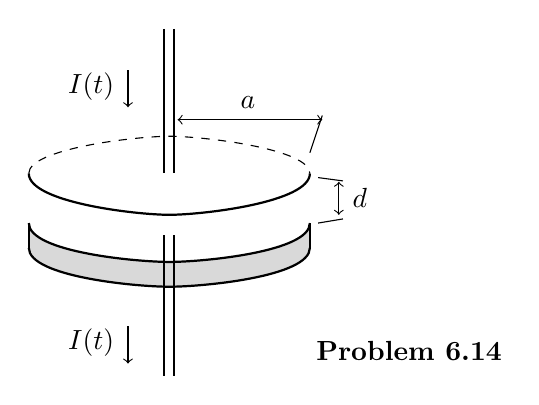
\begin{tikzpicture}[scale=1.05]
  % top plate (drawn as ellipse: flat rim, dashed back edge)
  \draw[thick] (-1.7,0.45) .. controls (-1.7,0.1) and (-0.4,-0.05) .. (0,-0.05)
               .. controls (0.4,-0.05) and (1.7,0.1) .. (1.7,0.45);
  \draw[dashed] (-1.7,0.45) .. controls (-1.7,0.75) and (-0.4,0.9) .. (0,0.9)
               .. controls (0.4,0.9) and (1.7,0.75) .. (1.7,0.45);
  % bottom plate: shaded side
  \fill[gray!30] (-1.7,-0.15) .. controls (-1.7,-0.5) and (-0.4,-0.62) .. (0,-0.62)
               .. controls (0.4,-0.62) and (1.7,-0.5) .. (1.7,-0.15)
               -- (1.7,-0.45) .. controls (1.7,-0.8) and (0.4,-0.92) .. (0,-0.92)
               .. controls (-0.4,-0.92) and (-1.7,-0.8) .. (-1.7,-0.45) -- cycle;
  \draw[thick] (-1.7,-0.15) .. controls (-1.7,-0.5) and (-0.4,-0.62) .. (0,-0.62)
               .. controls (0.4,-0.62) and (1.7,-0.5) .. (1.7,-0.15);
  \draw[thick] (-1.7,-0.45) .. controls (-1.7,-0.8) and (-0.4,-0.92) .. (0,-0.92)
               .. controls (0.4,-0.92) and (1.7,-0.8) .. (1.7,-0.45);
  \draw[thick] (-1.7,-0.15) -- (-1.7,-0.45);
  \draw[thick] (1.7,-0.15) -- (1.7,-0.45);
  % Separate axial leads terminate on their respective plates (source p. 289).
  \draw[thick] (0.06,2.2) -- (0.06,0.45);
  \draw[thick] (-0.06,2.2) -- (-0.06,0.45);
  \draw[thick] (0.06,-0.3) -- (0.06,-2.0);
  \draw[thick] (-0.06,-0.3) -- (-0.06,-2.0);
  % current arrows on the wire
  \draw[->] (-0.5,1.7) -- (-0.5,1.25);
  \node[left] at (-0.55,1.5) {$I(t)$};
  \draw[->] (-0.5,-1.4) -- (-0.5,-1.85);
  \node[left] at (-0.55,-1.6) {$I(t)$};
  % radius arrow a
  \draw[<->] (0.1,1.1) -- (1.85,1.1);
  \node[above] at (0.95,1.12) {$a$};
  \draw (1.7,0.7) -- (1.85,1.15);
  % gap arrow d
  \draw[<->] (2.05,0.35) -- (2.05,-0.05);
  \draw (1.8,0.4) -- (2.1,0.36);
  \draw (1.8,-0.15) -- (2.1,-0.1);
  \node[right] at (2.1,0.15) {$d$};
  \node at (2.9,-1.7) {\textbf{Problem 6.14}};
\end{tikzpicture}
\end{center}

\begin{enumerate}
\item[(a)] Calculate the electric and magnetic fields between the plates to second order in powers of the frequency (or wave number), neglecting the effects of fringing fields.
\item[(b)] Calculate the volume integrals of $w_{e}$ and $w_{m}$ that enter the definition of the reactance $X$, (6.140), \erratum{through second relative order in $\omega a/c$. (For absolute order $\omega^2$ at fixed current, the electric energy also needs the relative $(\omega a/c)^4/192$ correction derived below.)} Show that in terms of the input current $I_{i}$, defined by $I_{i}=-i\omega Q$, where $Q$ is the \emph{total charge} on one plate, these energies are
\[
\int w_{e}\;d^{3}x=\frac{1}{4\pi\epsilon_{0}}\frac{|I_{i}|^{2}d}{\omega^{2}a^{2}},\qquad
\int w_{m}\;d^{3}x=\frac{\mu_{0}}{4\pi}\frac{|I_{i}|^{2}d}{8}\left(1+\frac{\omega^{2}a^{2}}{12c^{2}}\right)
\]
\item[(c)] Show that the equivalent series circuit has $C\simeq\pi\epsilon_{0}a^{2}/d$, $L\simeq\mu_{0}d/8\pi$, and that an estimate for the resonant frequency of the system is $\omega_{\mathrm{res}}\simeq2\sqrt{2}\,c/a$. Compare with the first root of $J_{0}(x)$.
\end{enumerate}
\solution

Use cylindrical radius $s$ and the phasor convention $e^{-i\omega t}$.
Let $Q=\epsilon_0\int E_z\,da$ be the signed plate charge and
$I_i=-i\omega Q$. The axial leads end on their respective plates; there
is no conducting connection through the gap (as in the source sketch on
printed p.~289).

\textbf{(a)} Neglecting fringing, the fields are $E_z(s),H_\phi(s)$.
The curl equations give
\[
-\frac{dE_z}{ds}=i\omega\mu_0H_\phi,\qquad
\frac1s\frac d{ds}(sH_\phi)=-i\omega\epsilon_0E_z,
\qquad \frac1s(sE_z')'+k^2E_z=0.
\]
Regularity at $s=0$ selects $E_z=A J_0(ks)$. Since
$\int_0^a sJ_0(ks)ds=aJ_1(ka)/k$, charge normalization fixes
\[
\boxed{E_z(s)=\frac{I_i k}{-i\omega\,2\pi\epsilon_0aJ_1(ka)}J_0(ks),
\qquad H_\phi(s)=\frac{I_i}{2\pi aJ_1(ka)}J_1(ks).}
\]
Here $B_\phi=\mu_0H_\phi$, and the actual fields are the real parts
of the phasors times $e^{-i\omega t}$. For $ka\ll1$,
\begin{align*}
E_z&=\frac{I_i}{-i\omega\pi\epsilon_0a^2}
\left[1+k^2\left(\frac{a^2}{8}-\frac{s^2}{4}\right)+O(k^4a^4)\right],\\
H_\phi&=\frac{I_i s}{2\pi a^2}
\left[1+\frac{k^2}{8}(a^2-s^2)+O(k^4a^4)\right].
\end{align*}
In particular $2\pi aH_\phi(a)=I_i$ exactly; the field at the rim
contains the total displacement current.

\textbf{(b)} With $w_e=\epsilon_0|E|^2/4$ and $w_m=\mu_0|H|^2/4$,
$\langle s^2\rangle_{\rm disk}=a^2/2$ makes the relative $k^2$ correction
to $W_e$ vanish. For the magnetic integral,
\[
\int_0^a s^3\left[1+\frac{k^2}{4}(a^2-s^2)\right]ds
=\frac{a^4}{4}\left(1+\frac{k^2a^2}{12}\right).
\]
Thus the two displayed leading-order results in the question are
\[
W_e=\frac{|I_i|^2d}{4\pi\epsilon_0\omega^2a^2}[1+O((ka)^4)],\qquad
W_m=\frac{\mu_0|I_i|^2d}{32\pi}
\left[1+\frac{(ka)^2}{12}+O((ka)^4)\right].
\]
There is an ordering subtlety in the wording ``to second order in
$\omega$'': at fixed $I_i$, the leading electric energy is $O(\omega^{-2})$.
For its \emph{absolute} $O(\omega^2)$ term one must retain the relative
$k^4$ correction. The exact Bessel solution settles this without extending
the approximate Maxwell calculation. Writing $z=ka$ and taking Bessel
functions below at $z$,
\[
\int_0^a sJ_\nu(ks)^2\,ds
=\frac{a^2}{2}\left[J_\nu(z)^2-J_{\nu-1}(z)J_{\nu+1}(z)\right].
\]
For $\nu=0$, $J_{-1}=-J_1$ makes the bracket $J_0^2+J_1^2$;
for $\nu=1$ it is $J_1^2-J_0J_2$. The identity follows by
differentiating its right-hand side, using
$2J_\nu'=J_{\nu-1}-J_{\nu+1}$ and
$2\nu J_\nu/z=J_{\nu-1}+J_{\nu+1}$.
Substitution of the exact field amplitudes then gives
\begin{align*}
W_e&=\frac{|I_i|^2d}{4\pi\epsilon_0\omega^2a^2}
\frac{z^2(J_0^2+J_1^2)}{4J_1^2}
=\frac{|I_i|^2d}{4\pi\epsilon_0\omega^2a^2}
\left[1+\frac{z^4}{192}+O(z^6)\right],\\
W_m&=\frac{\mu_0|I_i|^2d}{16\pi}
\left[1-\frac{J_0J_2}{J_1^2}\right].
\end{align*}
The $z^4/192$ term is absent from the book's displayed $W_e$;
it is necessary if both energies are demanded through absolute order
$\omega^2$, but it does not affect the requested leading $L,C$.

\textbf{(c)} From $X=4\omega(W_m-W_e)/|I_i|^2$,
\[
X=-\frac1{\omega C}+\omega L+O(\omega^3),\qquad
\boxed{C=\frac{\pi\epsilon_0a^2}{d},\quad L=\frac{\mu_0d}{8\pi},\quad
\omega_{LC}=\frac1{\sqrt{LC}}=2\sqrt2\,\frac ca.}
\]
The exact energy difference, using $J_0+J_2=2J_1/z$, gives
\[
X=-\frac{\mu_0\omega d}{2\pi}\frac{J_0(z)}{zJ_1(z)}.
\]
Its first zero is $z=j_{0,1}=2.4048255577$, whereas
$2\sqrt2=2.8284271247$: the lumped estimate is $17.61\%$ too high.
This is expected because its putative resonance has $ka$ of order one,
outside the small-frequency expansion. Both results neglect edge and
lead effects; they describe the idealized gap field model.

\Needspace{5\baselineskip}
\par\bigskip
\noindent\textbf{6.15}\quad If a conductor or semiconductor has current flowing in it because of an applied electric field, and a transverse magnetic field is applied, there develops a component of electric field in the direction orthogonal to both the applied electric field (direction of current flow) and the magnetic field, resulting in a voltage difference between the sides of the conductor. This phenomenon is known as the \emph{Hall effect}.
\begin{enumerate}
\item[(a)] Use the known properties of electromagnetic fields under rotations and spatial reflections and the assumption of Taylor series expansions around zero magnetic field strength to show that for an isotropic medium the generalization of Ohm's law, correct to second order in the magnetic field, must have the form
\[
\mathbf{E}=\rho_{0}\mathbf{J}+R(\mathbf{H}\times\mathbf{J})+\beta_{1}H^{2}\mathbf{J}+\beta_{2}(\mathbf{H}\cdot\mathbf{J})\mathbf{H}
\]
where $\rho_{0}$ is the resistivity in the absence of the magnetic field and $R$ is called the Hall coefficient.
\item[(b)] What about the requirements of time reversal invariance?
\end{enumerate}
\solution

\textbf{(a)} Linear response to current means $E_i=\rho_{ij}(\mathbf H)J_j$.
For an isotropic medium the rank-two tensors that can be formed through
second order in the axial vector $\mathbf H$ are
\[
\rho_{ij}=\rho_0\delta_{ij}
+R\epsilon_{ikj}H_k+\beta_1H_kH_k\delta_{ij}+\beta_2H_iH_j+O(H^3).
\]
To see completeness, the zero-order isotropic tensor is $\delta_{ij}$;
the only rank-three isotropic pseudotensor is $\epsilon_{ikj}$; and the
three rank-four delta products, contracted with $H_kH_l$, reduce to
$H^2\delta_{ij}$ and $H_iH_j$. Under inversion $\mathbf E,\mathbf J$
are polar and $\mathbf H$ is axial, so all these terms transform as required.
Consequently
\[
\boxed{\mathbf E=\rho_0\mathbf J+R(\mathbf H\times\mathbf J)
+\beta_1H^2\mathbf J+\beta_2(\mathbf H\cdot\mathbf J)\mathbf H+O(H^3J).}
\]
The Hall part is antisymmetric and does no Joule work:
\[
\mathbf J\cdot\mathbf E=(\rho_0+\beta_1H^2)J_\perp^2
+[\rho_0+(\beta_1+\beta_2)H^2]J_\parallel^2.
\]
Passivity requires these two coefficients to be nonnegative over the field
range in which the expansion is used.

\textbf{(b)} Under time reversal $\mathbf E$ is even, whereas $\mathbf J$
and $\mathbf H$ are odd. Thus the Hall term is even, as required for a
reversible force balance, while the longitudinal dissipative terms are odd.
A resistive macroscopic law with a fixed sign of dissipation is not itself
invariant under reversal of a nonequilibrium history: heat flow and the
reservoir state must be reversed too. It would therefore be incorrect to
set $\rho_0,\beta_1,\beta_2$ to zero by applying time reversal directly to
Ohm's dissipative law.

Microscopic time-reversal symmetry in equilibrium instead implies the
Onsager--Casimir condition $\rho_{ij}(\mathbf H)=\rho_{ji}(-\mathbf H)$,
provided the magnetic field is the only time-reversal-odd bias and there
is no spontaneous magnetic order. The even-in-$H$ symmetric terms and
the odd-in-$H$ antisymmetric Hall term above all satisfy this condition.
It imposes no further relation among the four coefficients.

\Needspace{5\baselineskip}
\par\bigskip
\noindent\textbf{6.16}\quad\begin{enumerate}
\item[(a)] Calculate the force in newtons acting on a Dirac monopole of the minimum magnetic charge located a distance 0.5 \AA\ from and in the median plane of a magnetic dipole with dipole moment equal to one nuclear magneton ($e\hbar/2m_{p}$).
\item[(b)] Compare the force in part a with atomic forces such as the direct electrostatic force between charges (at the same separation), the spin-orbit force, the hyperfine interaction. Comment on the question of binding of magnetic monopoles to nuclei with magnetic moments. Assume that the monopole mass is at least that of a proton.
\end{enumerate}
\emph{Reference}: D. Sivers, \emph{Phys. Rev.} \textbf{D2}, 2048 (1970).
\solution

\textbf{(a)} In the SI convention of (6.153), $eg_D=2\pi\hbar$ and the
static force on a monopole is $g_D\mathbf H=g_D\mathbf B/\mu_0$.
For $\mathbf m=\mu_N\hat{\mathbf z}$, $\mu_N=e\hbar/(2m_p)$, the
\emph{median-plane} dipole field is
$\mathbf B=-\mu_0\mu_N\hat{\mathbf z}/(4\pi r^3)$. It is half the
magnitude of the axial dipole field. Therefore
\[
\mathbf F=-\frac{g_D\mu_N}{4\pi r^3}\hat{\mathbf z}
=-\frac{\hbar^2}{4m_pr^3}\hat{\mathbf z},\qquad
\boxed{|\mathbf F|=1.330\times10^{-11}\ {\rm N}\quad(r=0.5\ \text{\AA}).}
\]
Here $g_D=h/e=4.13567\times10^{-15}\ {\rm Wb}$; a negative monopole
reverses the force.

\textbf{(b)} The Coulomb force at the same separation is
\[
F_C=\frac{e^2}{4\pi\epsilon_0r^2}=9.228\times10^{-8}\ {\rm N},\qquad
\frac{|F|}{F_C}=\frac14\frac{m_e}{m_p}\frac{a_0}{r}
=1.441\times10^{-4}.
\]
Thus the monopole force is about $6940$ times smaller than the direct
atomic electric force. Atomic spin-orbit forces have the characteristic
relativistic scale $\alpha^2F_C\simeq4.91\times10^{-12}\ {\rm N}$ at the
same $r=0.5$~\AA${}\sim a_0$ (angular and state-dependent coefficients are not specified).
The monopole force is about $2.7$ times this scale. For a concrete
hyperfine comparison, two magnetic moments of magnitudes $\mu_B$ and
$\mu_N$ have dipolar energy scale
$\mu_0\mu_B\mu_N/(4\pi r^3)$ and radial force scale
\[
F_{\rm hf}\sim\frac{3\mu_0\mu_B\mu_N}{4\pi r^4}
=2.25\times10^{-15}\ {\rm N}.
\]
The monopole force is roughly $5900$ times this scale. These last two
comparisons are scales, not a claim that every atomic level has a
nonzero spin-orbit or hyperfine force.

The dipole--monopole potential is anisotropic:
\[
U(r,\theta)=\frac{g_D\mu_N}{4\pi r^2}\cos\theta
=\frac{\hbar^2}{4m_pr^2}\cos\theta.
\]
Here $\mathbf r$ points from the fixed dipole to the monopole. The energy
is negative on the $\cos\theta<0$ side and becomes strong at short
distance. Its characteristic magnitude at the stated atomic distance is
$|U|_{\rm scale}=4.15\times10^{-3}\ {\rm eV}$, but at a nuclear cutoff
$r_N$ the same point-dipole estimate grows as $r_N^{-2}$.
A localization kinetic-energy scale for relative mass $m_{\rm red}$ is
$\hbar^2/(2m_{\rm red}r^2)$, so their ratio for a moment of one nuclear
magneton is $m_{\rm red}/(2m_p)$. A heavy monopole and a heavy nucleus
can therefore make the attraction competitive with localization energy;
for a general moment the ratio is $(\mu/\mu_N)\,m_{\rm red}/(2m_p)$.
For an electron, $\mu_B=(m_p/m_e)\mu_N$ merely offsets its small reduced
mass, leaving a ratio of only about $1/2$, so electron binding is much
less favored than binding to a heavy magnetic nucleus.
Binding to suitable magnetic nuclei is consequently plausible despite
the weak force at atomic distances. A universal binding energy or a
proof of binding for every nucleus does not follow from this estimate:
spin, electric charge--monopole angular momentum, the actual nuclear
moment, and the finite nuclear core are required. The mass assumption
alone does not supply those data. In particular the attractive inverse
square potential has no intrinsic length scale, so a physical short-distance
model is indispensable for a binding energy.

\Needspace{5\baselineskip}
\par\bigskip
\noindent\textbf{6.17}\quad\begin{enumerate}
\item[(a)] For a particle possessing both electric and magnetic charges, show that the generalization of the Lorentz force in vacuum is
\[
\mathbf{F}=q_{\mathrm{e}}\mathbf{E}+q_{\mathrm{m}}\mathbf{B}/\mu_{0}+q_{\mathrm{e}}\mathbf{v}\times\mathbf{B}-q_{\mathrm{m}}\mathbf{v}\times\epsilon_{0}\mathbf{E}
\]
\item[(b)] Show that this expression for the force is invariant under a duality transformation of both fields and charges, (6.151) and (6.152).
\item[(c)] Show that the Dirac quantization condition, (6.153), is generalized for two particles possessing electric and magnetic charges $e_{1},g_{1}$ and $e_{2},g_{2}$, respectively, to
\[
\frac{e_{1}g_{2}-e_{2}g_{1}}{\hbar}=2\pi n
\]
and that the relation is invariant under a duality transformation of the charges.
\end{enumerate}
\solution

\textbf{(a)} Duality maps the electric force $q_e(\mathbf E+\mathbf v\times\mathbf B)$
to a magnetic-charge force. In vacuum put
$Z_0=\sqrt{\mu_0/\epsilon_0}=\mu_0c$, and use a quarter-turn of the
normalized field pair $(\mathbf E,c\mathbf B)$. The corresponding magnetic
force is
$q_m(\mathbf B/\mu_0-\epsilon_0\mathbf v\times\mathbf E)$.
Superposition therefore gives
\[
\boxed{\mathbf F=q_e\mathbf E+q_m\mathbf B/\mu_0
+q_e\mathbf v\times\mathbf B-q_m\epsilon_0\mathbf v\times\mathbf E.}
\]
This also has the required power $\mathbf F\cdot\mathbf v
=q_e\mathbf E\cdot\mathbf v+q_m\mathbf H\cdot\mathbf v$;
both velocity cross-product terms do no work.

\textbf{(b)} Express (6.151)--(6.152) as a common rotation by an arbitrary
angle $\chi$ (changing $\chi$ to $-\chi$ exchanges the book's primed/unprimed
convention):
\[
\begin{pmatrix}\mathbf E'\\c\mathbf B'\end{pmatrix}
=\begin{pmatrix}\cos\chi&\sin\chi\\-\sin\chi&\cos\chi\end{pmatrix}
\begin{pmatrix}\mathbf E\\c\mathbf B\end{pmatrix},\qquad
\begin{pmatrix}q_e'\\q_m'/Z_0\end{pmatrix}
=\begin{pmatrix}\cos\chi&\sin\chi\\-\sin\chi&\cos\chi\end{pmatrix}
\begin{pmatrix}q_e\\q_m/Z_0\end{pmatrix}.
\]
With $a=q_e$, $b=q_m/Z_0$, and $\mathbf F_1=\mathbf E$,
$\mathbf F_2=c\mathbf B$, the force is
\[
\mathbf F=a\mathbf F_1+b\mathbf F_2
+\frac{\mathbf v}{c}\times(a\mathbf F_2-b\mathbf F_1).
\]
The first combination is the scalar product of two pairs; the second is
their antisymmetric product. Both are preserved by a common rotation of
determinant one, proving force invariance including all factors of $c,Z_0$.

\textbf{(c)} Rotate particle 1 to a purely electric charge. If it is
nonzero, choose
\[
 e_1'=\sqrt{e_1^2+(g_1/Z_0)^2},\qquad g_1'=0.
\]
The determinant of the two charge vectors is invariant, so
$e_1'g_2'=e_1g_2-e_2g_1$. Applying the electric--magnetic Dirac condition
in that frame gives
\[
\boxed{e_1g_2-e_2g_1=2\pi n\hbar,\qquad n\in\mathbb Z.}
\]
If particle 1 carries neither charge the left side vanishes and $n=0$.
Equivalently, the two-source field angular momentum has coefficient
$(e_1g_2-e_2g_1)/(4\pi)$, whose allowed half-integral multiples of $\hbar$
give the same condition. The determinant argument proves its invariance
under every common duality transformation.

\Needspace{5\baselineskip}
\par\bigskip
\noindent\textbf{6.18}\quad Consider the Dirac expression
\[
\mathbf{A}(\mathbf{x})=\frac{g}{4\pi}\int_{L}\frac{d\mathbf{l}'\times(\mathbf{x}-\mathbf{x}')}{|\mathbf{x}-\mathbf{x}'|^{3}}
\]
for the vector potential of a magnetic monopole and its associated string $L$. Suppose for definiteness that the monopole is located at the origin and the string along the negative $z$ axis.
\begin{enumerate}
\item[(a)] Calculate $\mathbf{A}$ explicitly and show that in spherical coordinates it has components
\[
A_{r}=0,\qquad A_{\theta}=0,\qquad A_{\phi}=\frac{g(1-\cos\theta)}{4\pi r\sin\theta}=\left(\frac{g}{4\pi r}\right)\tan\!\left(\frac{\theta}{2}\right)
\]
\item[(b)] Verify that $\mathbf{B}=\nabla\times\mathbf{A}$ is the Coulomb-like field of a point charge, except perhaps at $\theta=\pi$.
\item[(c)] With the $\mathbf{B}$ determined in part b, evaluate the total magnetic flux passing through the circular loop of radius $R\sin\theta$ shown in the figure. Consider $\theta<\pi/2$ and $\theta>\pi/2$ separately, but always calculate the upward flux.
\item[(d)] From $\oint\mathbf{A}\cdot d\mathbf{l}$ around the loop, determine the total magnetic flux through the loop. Compare the result with that found in part c. Show that they are equal for $0<\theta<\pi/2$, but have a \emph{constant} difference for $\pi/2<\theta<\pi$. Interpret this difference.
\end{enumerate}

\begin{center}
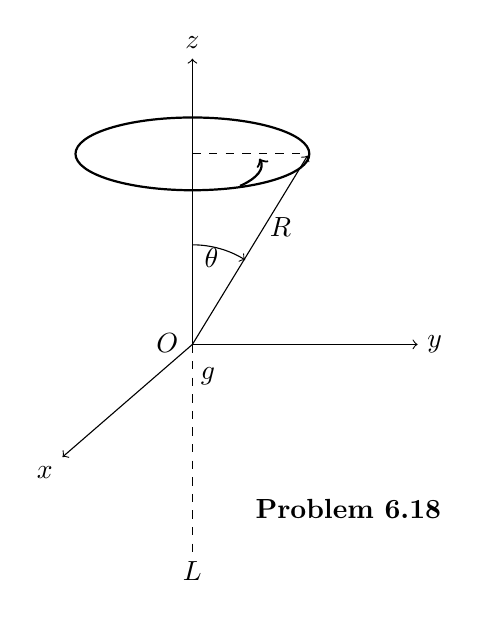
\begin{tikzpicture}[scale=1.1]
  % axes
  \draw[->] (0,0) -- (0,3.3) node[above] {$z$};
  \draw[->] (0,0) -- (2.6,0) node[right] {$y$};
  \draw[->] (0,0) -- (-1.5,-1.3) node[below left] {$x$};
  % dashed string along negative z to L
  \draw[dashed] (0,0) -- (0,-2.4) node[below] {$L$};
  % circular loop (ellipse) at height
  \draw[thick] (0,2.2) ellipse (1.35 and 0.42);
  % thick arrow on the front-right arc showing circulation direction
  \draw[->,thick] (0.55,1.83) arc (-35:10:1.35 and 0.42);
  % R vector from O to the right tip of the loop
  \draw[->] (0,0) -- (1.33,2.18);
  \node[right] at (0.78,1.35) {$R$};
  % theta angle between z axis and R
  \draw[->] (0,1.15) arc (90:58:1.15);
  \node at (0.22,1.0) {$\theta$};
  % origin and g label
  \node[left] at (-0.05,0.02) {$O$};
  \node[below] at (0.18,-0.15) {$g$};
  % dashed radius of the loop (R sin theta)
  \draw[dashed] (0,2.2) -- (1.35,2.2);
  \node at (1.8,-1.9) {\textbf{Problem 6.18}};
\end{tikzpicture}
\end{center}
\solution

\textbf{(a)} Parameterize the string by $\mathbf x'=z'\hat{\mathbf z}$,
$-\infty<z'\le0$, with $d\mathbf l'=\hat{\mathbf z}\,dz'$. Its numerator
is $d\mathbf l'\times(\mathbf x-\mathbf x')=s\hat{\boldsymbol\phi}\,dz'$,
where $s=r\sin\theta$. Thus
\begin{align*}
A_\phi&=\frac g{4\pi}\int_{-\infty}^0
\frac{s\,dz'}{[s^2+(z-z')^2]^{3/2}}\\
&=\frac g{4\pi s}\left(1-\frac z{\sqrt{s^2+z^2}}\right)
=\boxed{\frac g{4\pi r}\frac{1-\cos\theta}{\sin\theta}
=\frac g{4\pi r}\tan\frac\theta2}.
\end{align*}
The other components vanish. This potential is regular on the positive
axis and singular on the negative axis.

\textbf{(b)} Away from that string,
\[
B_r=\frac1{r\sin\theta}\partial_\theta(\sin\theta A_\phi)
=\frac g{4\pi r^2},\qquad
B_\theta=-\frac1r\partial_r(rA_\phi)=0,\qquad B_\phi=0.
\]
Thus the ordinary curl is the monopole field
$\boxed{\mathbf B=g\hat{\mathbf r}/(4\pi r^2)}$ off the string and origin.

\textbf{(c)} The horizontal disk lies at $z_0=R\cos\theta$, with radius
$s_0=R\sin\theta$. For $z_0\ne0$ its upward monopole flux is
\begin{align*}
\Phi_{\rm mono}^{\uparrow}
&=\frac g2\int_0^{s_0}\frac{z_0s\,ds}{(s^2+z_0^2)^{3/2}}
=\frac g2\left[\operatorname{sgn}(z_0)-\frac{z_0}{R}\right]\\
&=\boxed{\begin{cases}
\frac g2(1-\cos\theta),&0<\theta<\pi/2,\\
-\frac g2(1+\cos\theta),&\pi/2<\theta<\pi.
\end{cases}}
\end{align*}
The disk at $\theta=\pi/2$ passes through the monopole and requires a
singular-surface prescription; it is excluded from these two cases.

\textbf{(d)} Counterclockwise circulation viewed from above gives
\[
\oint\mathbf A\cdot d\mathbf l=2\pi R\sin\theta\,A_\phi(R,\theta)
=\boxed{\frac g2(1-\cos\theta)}.
\]
It equals the flux in part (c) for the upper disk, but exceeds that flux
by $g$ for the lower disk. The distributional curl includes a return-flux
string:
\[
\nabla\times\mathbf A=\frac g{4\pi r^2}\hat{\mathbf r}
+g\delta(x)\delta(y)\Theta(-z)\hat{\mathbf z}.
\]
Its upward flux through every disk cutting the negative axis is $g$.
Its divergence is $-g\delta^{(3)}(\mathbf x)$, which cancels the monopole
field's divergence, as every globally defined distributional curl must.
Excluding the string gives the isolated monopole field; retaining it
restores Stokes's theorem for disks crossing the string.

\Needspace{5\baselineskip}
\par\bigskip
\noindent\textbf{6.19}\quad\begin{enumerate}
\item[(a)] Apply space inversion to the monopole vector potential of Problem 6.18 and show that the vector potential becomes
\[
A'_{\phi}=-g\frac{(1+\cos\theta)}{4\pi r\,\sin\theta}=-\frac{g}{4\pi r}\cot\!\left(\frac{\theta}{2}\right)
\]
with the other components vanishing. Show explicitly that its curl gives the magnetic field of a magnetic monopole, except perhaps at $\theta=0$. [Remember the space-inversion properties of the magnetic charge!]
\item[(b)] Show that the difference, $\delta\mathbf{A}=\mathbf{A}'-\mathbf{A}$, can be expressed as the gradient of a scalar function, indicating that the original and space-inverted vector potentials differ by a gauge transformation.
\item[(c)] Interpret the gauge function in terms of Fig.~6.9. [\emph{Hint}: Choose the contour $C$ to be a rectangle lying in a plane containing the $z$ axis, with three sides at infinity.]
\end{enumerate}
\solution

\textbf{(a)} A vector potential is a polar vector, so under active parity
$\mathbf A^P(\mathbf x)=-\mathbf A(-\mathbf x)$, whereas magnetic charge
is a pseudoscalar, $g^P=-g$. At $-\mathbf x$, the angles are
$(\pi-\theta,\phi+\pi)$ and $\hat{\boldsymbol\phi}(\phi+\pi)
=-\hat{\boldsymbol\phi}(\phi)$. Applying these facts to 6.18 gives
\[
\mathbf A^P(\mathbf x)=\frac{g(1+\cos\theta)}{4\pi r\sin\theta}
\hat{\boldsymbol\phi}
=-\frac{g^P(1+\cos\theta)}{4\pi r\sin\theta}\hat{\boldsymbol\phi}.
\]
Now denote the \emph{transformed} monopole charge by $g$, as in the question.
The potential of that charge with its string on the positive axis is
\[
\boxed{A'_\phi=-\frac{g(1+\cos\theta)}{4\pi r\sin\theta}
=-\frac g{4\pi r}\cot\frac\theta2,\qquad A'_r=A'_\theta=0.}
\]
Direct differentiation gives
$B'_r=(r\sin\theta)^{-1}\partial_\theta(\sin\theta A'_\phi)
=g/(4\pi r^2)$ and $B'_\theta=B'_\phi=0$ away from the positive-axis
string. Keeping the original pre-parity charge label instead gives a
monopole of charge $-g$, consistently with its pseudoscalar character.

\textbf{(b)} Comparing potentials of the \emph{same} charge $g$ on their
common nonsingular domain,
\[
\delta\mathbf A=-\frac g{2\pi r\sin\theta}\hat{\boldsymbol\phi}
=\nabla\Lambda,\qquad
\boxed{\Lambda=-\frac g{2\pi}\phi+\hbox{constant}.}
\]
Since $\nabla\phi=\hat{\boldsymbol\phi}/(r\sin\theta)$, this is a gauge
transformation on a patch with a chosen azimuthal cut. The scalar is not
globally single-valued: $\phi\mapsto\phi+2\pi$ changes it by $-g$.
The quantum phase $\exp(i e\Lambda/\hbar)$ is nevertheless single-valued
when $eg=2\pi n\hbar$.

\textbf{(c)} In Fig.~6.9 the contour is $C=L'-L$. For strings on opposite
halves of the $z$ axis, close this contour with three sides of a rectangle
at infinity in a meridian plane. Its spanning surface becomes a half-plane
ending on the axis. On a unit sphere centered at the observer, a change
$d\phi$ sweeps out a spherical lune. Its unsigned area is
\[
\int_\phi^{\phi+d\phi}d\varphi\int_0^\pi\sin\vartheta\,d\vartheta
=2\,d\phi.
\]
The contour orientation $C=L'-L$ assigns the negative sign, so the
oriented solid angle changes by $-2\,d\phi$.
Thus, on a chosen branch,
\[
\Omega_C=-2\phi+\hbox{constant},\qquad
\Lambda=\frac g{4\pi}\Omega_C.
\]
This is exactly Jackson's (6.162). Crossing the half-plane changes the
solid-angle branch by $4\pi$, or the gauge function by $g$ in magnitude;
that jump represents relocation of the unobservable string.

\Needspace{5\baselineskip}
\par\bigskip
\noindent\textbf{6.20}\quad An example of the preservation of causality and finite speed of propagation in spite of the use of the Coulomb gauge is afforded by a dipole source that is flashed on and off at $t=0$. The effective charge and current densities are
\begin{align*}
\rho(\mathbf{x},t)&=\delta(x)\delta(y)\delta'(z)\delta(t)\\
J_{z}(\mathbf{x},t)&=-\delta(x)\delta(y)\delta(z)\delta'(t)
\end{align*}
where a prime means differentiation with respect to the argument. This dipole is of unit strength and it points in the negative $z$ direction.
\begin{enumerate}
\item[(a)] Show that the instantaneous Coulomb potential (6.23) is
\[
\Phi(\mathbf{x},t)=-\frac{1}{4\pi\epsilon_{0}}\;\delta(t)\;\frac{z}{r^{3}}
\]
\item[(b)] Show that the \emph{transverse} current $\mathbf{J}_{t}$ is
\[
\mathbf{J}_{t}(\mathbf{x},t)=-\delta'(t)\!\left[\tfrac{2}{3}\boldsymbol{\epsilon}_{3}\delta(\mathbf{x})-\frac{\boldsymbol{\epsilon}_{3}}{4\pi r^{3}}+\frac{3}{4\pi r^{3}}\,\mathbf{n}(\boldsymbol{\epsilon}_{3}\cdot\mathbf{n})\right]
\]
where the factor of 2/3 multiplying the delta function comes from treating the gradient of $z/r^{3}$ according to (4.20).
\item[(c)] Show that the electric and magnetic fields are causal and that the electric field components are
\[
E_{x}(\mathbf{x},t)=\frac{1}{4\pi\epsilon_{0}}\frac{c}{r}\left[-\delta''(r-ct)+\frac{3}{r}\delta'(r-ct)-\frac{3}{r^{2}}\delta(r-ct)\right]\sin\theta\cos\theta\cos\phi
\]
$E_{y}$ is the same as $E_{x}$, with $\cos\phi$ replaced by $\sin\phi$, and
\[
E_{z}(\mathbf{x},t)=\frac{1}{4\pi\epsilon_{0}}\frac{c}{r}\left[\sin^{2}\theta\,\delta''(r-ct)+(3\cos^{2}\theta-1)\cdot\left(\frac{\delta'(r-ct)}{r}-\frac{\delta(r-ct)}{r^{2}}\right)\right]
\]
\end{enumerate}
\emph{Hint}: While the answer in part b displays the transverse current explicitly, the less explicit form
\[
\mathbf{J}_{t}(\mathbf{x},t)=-\delta'(t)\!\left[\boldsymbol{\epsilon}_{3}\delta(\mathbf{x})+\frac{1}{4\pi}\nabla\frac{\partial}{\partial z}\left(\frac{1}{r}\right)\right]
\]
can be used with (6.47) to calculate the vector potential and the fields for part c. An alternative method is to use the Fourier transforms in time of $\mathbf{J}_{t}$ and $\mathbf{A}$, the Green function (6.40) and its spherical wave expansion from Chapter 9.
\solution

All fields below are distributions, and the explicit spherical formulas
are for $r>0$. Let $K=1/(4\pi\epsilon_0)$ and
$\mathbf e_z=\boldsymbol\epsilon_3$.

\textbf{(a)} Integrating the derivative of the source delta function gives
\[
\Phi_C=K\delta(t)\int\frac{\delta(x')\delta(y')\delta'(z')}
{|\mathbf x-\mathbf x'|}\,d^3x'
=-K\delta(t)\left.\partial_{z'}\frac1{|\mathbf x-\mathbf x'|}\right|_0
=\boxed{-K\delta(t)\frac z{r^3}}.
\]

\textbf{(b)} Charge conservation and $\nabla^2\Phi_C=-\rho/\epsilon_0$
show that the longitudinal current is
$\mathbf J_\ell=\epsilon_0\nabla\partial_t\Phi_C$.
Consequently
\[
\mathbf J_t=\mathbf J-\mathbf J_\ell
=-\delta'(t)\left[\mathbf e_z\delta^{(3)}(\mathbf x)
+\frac1{4\pi}\nabla\partial_z\frac1r\right].
\]
The distributional derivative checked in (4.20) is
\[
\partial_i\partial_j\frac1r
=\frac{3n_in_j-\delta_{ij}}{r^3}
-\frac{4\pi}{3}\delta_{ij}\delta^{(3)}(\mathbf x),
\]
where the $r^{-3}$ expression uses spherical principal-value exclusion.
It changes the contact term from $1$ to $2/3$ and yields
\[
\boxed{\mathbf J_t=-\delta'(t)\left[
\frac23\mathbf e_z\delta^{(3)}(\mathbf x)
-\frac{\mathbf e_z}{4\pi r^3}
+\frac{3\mathbf n n_z}{4\pi r^3}\right].}
\]
Taking a divergence of the less explicit form gives zero, since
$\nabla^2(1/r)=-4\pi\delta^{(3)}(\mathbf x)$.

\textbf{(c)} One can display the instantaneous cancellation without
integrating the spatially nonlocal $\mathbf J_t$ directly. The source is
an electric dipole $\mathbf p(t)=-\mathbf e_z\delta(t)$. Applying the
retarded potential integral (6.47) to the source deltas gives the Lorenz-gauge
potentials, with $\tau=t-r/c$,
\[
\Phi_L=-K n_z\left[\frac{\delta(\tau)}{r^2}
+\frac{\delta'(\tau)}{cr}\right],\qquad
\mathbf A_L=-\frac K{c^2r}\mathbf e_z\delta'(\tau).
\]
For example, the second term in $\Phi_L$ is the derivative of the retarded
time when the source-coordinate derivative acts on the delta function.
Define
\[
\chi=K n_z\left[\frac{\Theta(t)-\Theta(\tau)}{r^2}
-\frac{\delta(\tau)}{cr}\right],\qquad
\mathbf A_C=\mathbf A_L+\nabla\chi.
\]
Direct differentiation gives $\partial_t\chi=\Phi_L-\Phi_C$.
For the spatial check write $\chi=K n_zF$,
$H=\Theta(t)-\Theta(\tau)$, and $F=H/r^2-\delta(\tau)/(cr)$.
Using $\partial_r H=\delta(\tau)/c$ gives
\[
F'=-\frac{2H}{r^3}+\frac{2\delta(\tau)}{cr^2}
+\frac{\delta'(\tau)}{c^2r},\qquad
F''+\frac{2F'}r-\frac{2F}{r^2}
=-\frac{\delta'(\tau)}{c^2r^2}-\frac{\delta''(\tau)}{c^3r}.
\]
The last expression times $K n_z$ is
$-\nabla\cdot\mathbf A_L$. Thus
$\nabla^2\chi=-\nabla\cdot\mathbf A_L$, so $\mathbf A_C$ is the
Coulomb-gauge potential; both statements include the source distributions.
Therefore
\[
-\nabla\Phi_C-\partial_t\mathbf A_C
=-\nabla\Phi_C-\partial_t\mathbf A_L-\nabla(\Phi_L-\Phi_C)
=-\nabla\Phi_L-\partial_t\mathbf A_L.
\]
The instantaneous Coulomb term cancels explicitly. Differentiating the
retarded potentials at $r>0$ yields
\begin{align*}
\mathbf E&=K\left[(\mathbf e_z-3\mathbf n n_z)
\left(\frac{\delta(\tau)}{r^3}+\frac{\delta'(\tau)}{cr^2}\right)
+(\mathbf e_z-\mathbf n n_z)\frac{\delta''(\tau)}{c^2r}\right],\\
\mathbf B&=-\frac{\mu_0}{4\pi}(\mathbf e_z\times\mathbf n)
\left[\frac{\delta'(\tau)}{r^2}+\frac{\delta''(\tau)}{cr}\right].
\end{align*}
Set $u=r-ct$. The distribution identities
$\delta(\tau)=c\delta(u)$, $\delta'(\tau)=-c^2\delta'(u)$, and
$\delta''(\tau)=c^3\delta''(u)$ give
\begin{align*}
\boxed{E_x}&=\boxed{\frac{Kc}{r}n_xn_z
\left[-\delta''(u)+\frac3r\delta'(u)-\frac3{r^2}\delta(u)\right]},\\
E_y&=\frac{Kc}{r}n_yn_z
\left[-\delta''(u)+\frac3r\delta'(u)-\frac3{r^2}\delta(u)\right],\\
\boxed{E_z}&=\boxed{\frac{Kc}{r}\left[(1-n_z^2)\delta''(u)
+(3n_z^2-1)\left(\frac{\delta'(u)}r-\frac{\delta(u)}{r^2}\right)\right]},\\
\mathbf B&=\frac{\mu_0c^2}{4\pi r}\sin\theta
\left[\frac{\delta'(u)}r-\delta''(u)\right]\hat{\boldsymbol\phi}.
\end{align*}
Substituting $n_x=\sin\theta\cos\phi$, $n_y=\sin\theta\sin\phi$,
$n_z=\cos\theta$ proves all requested components. Every field at $r>0$
has support only on $r=ct$, $t>0$; the nonlocal Coulomb-gauge potentials
have produced a causal flash with finite speed $c$.

\Needspace{5\baselineskip}
\par\bigskip
\noindent\textbf{6.21}\quad An electric dipole of dipole moment $\mathbf{p}$, fixed in direction \erratum{and magnitude}, is located at a position $\mathbf{r}_{0}(t)$ with respect to the origin. Its velocity $\mathbf{v}=d\mathbf{r}_{0}/dt$ is nonrelativistic.
\begin{enumerate}
\item[(a)] Show that the dipole's charge and current densities can be expressed formally as
\[
\rho(\mathbf{x},t)=-(\mathbf{p}\cdot\nabla)\delta(\mathbf{x}-\mathbf{r}_{0}(t));\qquad
\mathbf{J}(\mathbf{x},t)=-\mathbf{v}(\mathbf{p}\cdot\nabla)\delta(\mathbf{x}-\mathbf{r}_{0}(t))
\]
\item[(b)] Show that the off-center moving dipole gives rise to a magnetic dipole field and an electric quadrupole field in addition to an electric dipole field, with moments
\[
\mathbf{m}=\tfrac{1}{2}\mathbf{p}\times\mathbf{v}
\]
and
\[
Q_{ij}=3(x_{0i}p_{j}+x_{0j}p_{i})-2\mathbf{r}_{0}\cdot\mathbf{p}\,\delta_{ij}
\]
[There are, of course, still higher moments.]
\item[(c)] Show that the quasi-static electric quadrupole field is
\[
\mathbf{E}(\mathbf{x})=\frac{1}{4\pi\epsilon_{0}}\frac{1}{r^{4}}\left[15\mathbf{n}(\mathbf{n}\cdot\mathbf{r}_{0})(\mathbf{n}\cdot\mathbf{p})-3\mathbf{r}_{0}(\mathbf{n}\cdot\mathbf{p})-3\mathbf{p}(\mathbf{n}\cdot\mathbf{r}_{0})-3\mathbf{n}(\mathbf{r}_{0}\cdot\mathbf{p})\right]
\]
where $\mathbf{n}$ is a unit vector in the radial direction.
\end{enumerate}
\solution

Take $\mathbf p$ to be constant in magnitude as well as direction. If only
its direction were fixed while its magnitude varied, the displayed current
would need an additional $\dot{\mathbf p}\delta(\mathbf x-\mathbf r_0)$.
The following derivation makes this assumption explicit.

\textbf{(a)} Represent the dipole by $+q$ at $\mathbf r_0+\mathbf d/2$
and $-q$ at $\mathbf r_0-\mathbf d/2$, translating with the common velocity
$\mathbf v$, and let $\mathbf p=q\mathbf d$ be fixed as $d\to0$.
Expansion of the two deltas gives
\[
\rho=q[\delta(\mathbf x-\mathbf r_0-\mathbf d/2)
-\delta(\mathbf x-\mathbf r_0+\mathbf d/2)]
\longrightarrow\boxed{-\mathbf p\cdot\nabla\delta(\mathbf x-\mathbf r_0)},
\qquad \boxed{\mathbf J=\mathbf v\rho}.
\]
Since $\partial_t\delta(\mathbf x-\mathbf r_0)=-\mathbf v\cdot\nabla\delta$,
these expressions satisfy $\partial_t\rho+\nabla\cdot\mathbf J=0$.

\textbf{(b)} For any smooth test function $F$,
\[
\int F\rho\,d^3x=p_k\partial_kF(\mathbf r_0).
\]
Taking $F=1,x_i$ gives zero net charge and electric moment $\mathbf p$.
For the magnetic moment,
\[
 m_i=\frac12\epsilon_{ijk}\int x_jv_k\rho\,d^3x
=\frac12\epsilon_{ijk}p_jv_k,\qquad
\boxed{\mathbf m=\tfrac12\mathbf p\times\mathbf v}.
\]
For the electric quadrupole use $F=3x_ix_j-r^2\delta_{ij}$:
\[
\boxed{Q_{ij}=p_k\partial_k(3x_ix_j-r^2\delta_{ij})\big|_{\mathbf r_0}
=3(x_{0i}p_j+x_{0j}p_i)-2(\mathbf r_0\cdot\mathbf p)\delta_{ij}}.
\]
Its trace vanishes. A moving off-center dipole generally has further
moments; neither formula assumes their absence.

\textbf{(c)} The quadrupole term in the far-zone, quasistatic potential is
\[
\Phi_Q=\frac1{4\pi\epsilon_0}\frac{Q_{ij}n_in_j}{2r^3}
=\frac1{4\pi\epsilon_0}\left[
\frac{3(\mathbf r_0\cdot\mathbf x)(\mathbf p\cdot\mathbf x)}{r^5}
-\frac{\mathbf r_0\cdot\mathbf p}{r^3}\right].
\]
Use $\nabla r^{-s}=-s\mathbf n r^{-s-1}$ and the product rule for the
quadratic numerator. Its negative gradient is
\[
\boxed{\mathbf E_Q=\frac1{4\pi\epsilon_0r^4}
\left[15\mathbf n(\mathbf n\cdot\mathbf r_0)(\mathbf n\cdot\mathbf p)
-3\mathbf r_0(\mathbf n\cdot\mathbf p)-3\mathbf p(\mathbf n\cdot\mathbf r_0)
-3\mathbf n(\mathbf r_0\cdot\mathbf p)\right].}
\]
This is the $r^{-4}$ term of the field expanded about the origin,
valid for $r\gg|\mathbf r_0|$; it is not the entire translated dipole field.

\Needspace{5\baselineskip}
\par\bigskip
\noindent\textbf{6.22}\quad\begin{enumerate}
\item[(a)] For the off-center, slowly moving, electric dipole of Problem 6.21, show that \erratum{the leading term for $r\gg|\mathbf r_0|$ in} the quasi-static vector potential produced by the current flow associated with the dipole motion is
\[
\mathbf{A}(\mathbf{x},t)=\frac{\mu_{0}\mathbf{v}(\mathbf{n}\cdot\mathbf{p})}{4\pi r^{2}}=\frac{\mu_{0}}{4\pi}\left[\frac{1}{2}\frac{(\mathbf{p}\times\mathbf{v})\times\mathbf{x}}{r^{3}}+\frac{1}{2}\frac{[\mathbf{p}(\mathbf{x}\cdot\mathbf{v})+\mathbf{v}(\mathbf{x}\cdot\mathbf{p})]}{r^{3}}\right]
\]
where the first term of the second form (antisymmetric in $\mathbf{v}$ and $\mathbf{p}$) is the vector potential of the magnetic dipole whose moment is given in Problem 6.21. The added term is symmetric in $\mathbf{v}$ and $\mathbf{p}$.
\item[(b)] Show that the magnetic field of the symmetric term is
\[
\mathbf{B}_{\mathrm{sym}}=-\frac{3\mu_{0}}{8\pi r^{3}}\,\mathbf{n}\times[\mathbf{p}(\mathbf{v}\cdot\mathbf{n})+\mathbf{v}(\mathbf{p}\cdot\mathbf{n})]
\]
\item[(c)] By calculating its curl, show that $\mathbf{B}_{\mathrm{sym}}$ is consistent with being the quasi-static magnetic field associated with the electric quadrupole field of Problem 6.21c.
\item[(d)] Show that the total magnetic field (computed from the first form of the vector potential, i.e., the sum of $\mathbf{B}_{\mathrm{sym}}$ and the magnetic \emph{dipole} field) is
\[
\mathbf{B}=\frac{\mu_{0}}{4\pi}\,\mathbf{v}\times\frac{[3\mathbf{n}(\mathbf{n}\cdot\mathbf{p})-\mathbf{p}]}{r^{3}}
\]
Comment.
\end{enumerate}
\solution

Keep the leading far-zone term in $|\mathbf r_0|/r$, and first order in
$v/c$, for the constant dipole moment of 6.21. A quasistatic observation
also requires retardation across the source and observer distance to be
small on the variation time scale.

\textbf{(a)} Direct integration of the derivative source gives the
instantaneous potential before expanding in $r_0/r$:
\[
\mathbf A(\mathbf x,t)=\frac{\mu_0\mathbf v}{4\pi}
\frac{\mathbf p\cdot(\mathbf x-\mathbf r_0)}{|\mathbf x-\mathbf r_0|^3}.
\]
Its leading term is
$\mu_0\mathbf v(\mathbf p\cdot\mathbf x)/(4\pi r^3)$, as stated.
The triple-product identity
$(\mathbf p\times\mathbf v)\times\mathbf x
=\mathbf v(\mathbf p\cdot\mathbf x)-\mathbf p(\mathbf v\cdot\mathbf x)$
splits it exactly into
\[
\boxed{\mathbf A=\frac{\mu_0}{8\pi r^3}
\left[(\mathbf p\times\mathbf v)\times\mathbf x
+\mathbf p(\mathbf v\cdot\mathbf x)+\mathbf v(\mathbf p\cdot\mathbf x)\right]}.
\]
The first term is the potential of $\mathbf m=\mathbf p\times\mathbf v/2$.

\textbf{(b)} Let $\mathbf C=\mathbf p(\mathbf v\cdot\mathbf x)
+\mathbf v(\mathbf p\cdot\mathbf x)$. Its curl vanishes, since the two
constant-vector cross products cancel. Therefore
\[
\mathbf B_{\rm sym}=\frac{\mu_0}{8\pi}\nabla(r^{-3})\times\mathbf C
=\boxed{-\frac{3\mu_0}{8\pi r^3}\mathbf n\times
[\mathbf p(\mathbf v\cdot\mathbf n)+\mathbf v(\mathbf p\cdot\mathbf n)]}.
\]

\textbf{(c)} Component differentiation using
$\partial_i n_j=(\delta_{ij}-n_in_j)/r$ gives
\[
\nabla\times\mathbf B_{\rm sym}
=\frac{\mu_0}{4\pi r^4}\left[
15\mathbf n(\mathbf n\cdot\mathbf v)(\mathbf n\cdot\mathbf p)
-3\mathbf v(\mathbf n\cdot\mathbf p)-3\mathbf p(\mathbf n\cdot\mathbf v)
-3\mathbf n(\mathbf v\cdot\mathbf p)\right].
\]
For an explicit way to organize the differentiation, use
$\nabla\times(\nabla\times\mathbf A_{\rm sym})
=\nabla(\nabla\cdot\mathbf A_{\rm sym})-\nabla^2\mathbf A_{\rm sym}$;
each $x_j/r^3$ is harmonic for $r>0$, so the Laplacian vanishes, and
\[
\nabla\cdot\mathbf A_{\rm sym}
=\frac{\mu_0}{4\pi}\left[
\frac{\mathbf p\cdot\mathbf v}{r^3}
-\frac{3(\mathbf p\cdot\mathbf x)(\mathbf v\cdot\mathbf x)}{r^5}\right].
\]
Its gradient is the displayed curl. Taking $\partial_t$ of 6.21(c)
replaces $\mathbf r_0$ by $\mathbf v$, hence
\[
\boxed{\nabla\times\mathbf B_{\rm sym}=\mu_0\epsilon_0\partial_t\mathbf E_Q.}
\]
This is exactly the source-free Amp\`ere--Maxwell equation at the retained
multipole order. The magnetic dipole field has zero curl for $r>0$ and
therefore cannot supply this displacement current by itself.

\textbf{(d)} Curl the unsplit potential:
\[
\mathbf B=\frac{\mu_0}{4\pi}\nabla\left(\frac{\mathbf p\cdot\mathbf x}{r^3}\right)
\times\mathbf v
=\boxed{\frac{\mu_0}{4\pi r^3}\mathbf v\times
[3\mathbf n(\mathbf n\cdot\mathbf p)-\mathbf p]}.
\]
It equals $\mathbf v\times\mathbf E_{\rm dip}/c^2$, the first-order
magnetic field generated by translating an electric dipole. The magnetic
dipole moment alone gives only part of it; the symmetric potential and
its electric-quadrupole displacement current are essential for the full
field. The exact instantaneous expression uses $\mathbf x-\mathbf r_0$
instead of $\mathbf x$, as shown in part (a).

\Needspace{5\baselineskip}
\par\bigskip
\noindent\textbf{6.23}\quad The wave equations (6.168) for the Hertz vectors contain arbitrary source terms involving the functions $\mathbf{V}$ and $\xi$. Consider the gauge transformations
\[
\boldsymbol{\Pi}_{\mathrm{e}}'=\boldsymbol{\Pi}_{\mathrm{e}}+\mu_{0}\nabla\times\mathbf{G}-\nabla g;\qquad
\boldsymbol{\Pi}_{\mathrm{m}}'=\boldsymbol{\Pi}_{\mathrm{m}}-\mu\frac{\partial\mathbf{G}}{\partial t}
\]
where $\mathbf{G}$ and $g$ are well-behaved functions of space and time.
\begin{enumerate}
\item[(a)] Show that, if $\mathbf{G}$ and $g$ satisfy the wave equations
\[
\left(\mu\epsilon\frac{\partial^{2}}{\partial t^{2}}-\nabla^{2}\right)\begin{Bmatrix}\mathbf{G}\\ g\end{Bmatrix}
=\begin{Bmatrix}\dfrac{1}{\mu}(\mathbf{V}+\nabla\xi)\\[8pt] 0\end{Bmatrix}
\]
then the new polarization potentials $\boldsymbol{\Pi}_{\mathrm{e}}'$ and $\boldsymbol{\Pi}_{\mathrm{m}}'$ satisfy (6.168) with vanishing $\mathbf{V}$ and $\xi$.
\item[(b)] Show that the gauge transformation on the Hertz vectors is equivalent to a gauge transformation on $\mathbf{A}$ and $\Phi$. What is the gauge function $\Lambda$ of (6.19) in terms of $\mathbf{G}$ and $g$?
\end{enumerate}
\solution

Let $\mathcal D=\mu\epsilon\partial_t^2-\nabla^2$, with constant
$\epsilon,\mu$. The actual equations (6.168), including their signs, are
\[
\mathcal D\boldsymbol\Pi_e=\mathbf P_{\rm ext}
-\frac{\mu_0}{\mu}\nabla\times\mathbf V,\qquad
\mathcal D\boldsymbol\Pi_m=\mathbf M_{\rm ext}
+\partial_t\mathbf V+\nabla\partial_t\xi.
\]

\textbf{(a)} Constant-coefficient derivatives commute with $\mathcal D$.
Apply it to the proposed transformed vectors and insert
$\mathcal D\mathbf G=(\mathbf V+\nabla\xi)/\mu$,
$\mathcal Dg=0$:
\begin{align*}
\mathcal D\boldsymbol\Pi'_e
&=\mathbf P_{\rm ext}-\frac{\mu_0}{\mu}\nabla\times\mathbf V
+\frac{\mu_0}{\mu}\nabla\times(\mathbf V+\nabla\xi)
-\nabla\mathcal Dg
=\boxed{\mathbf P_{\rm ext}},\\
\mathcal D\boldsymbol\Pi'_m
&=\mathbf M_{\rm ext}+\partial_t(\mathbf V+\nabla\xi)
-\partial_t(\mathbf V+\nabla\xi)
=\boxed{\mathbf M_{\rm ext}}.
\end{align*}
These are (6.168) with both arbitrary source functions set to zero.

\textbf{(b)} Equation (6.166) defines
\[
\mathbf A=\mu\partial_t\boldsymbol\Pi_e+\mu_0\nabla\times\boldsymbol\Pi_m,
\qquad \Phi=-\epsilon^{-1}\nabla\cdot\boldsymbol\Pi_e.
\]
The $\mathbf G$ contributions cancel identically in $\mathbf A$, while
its divergence contribution to $\Phi$ is zero. The remaining changes are
\[
\delta\mathbf A=-\mu\nabla\partial_tg,\qquad
\delta\Phi=\epsilon^{-1}\nabla^2g=\mu\partial_t^2g,
\]
where the last equality uses $\mathcal Dg=0$. Thus
\[
\boxed{\Lambda=-\mu\partial_tg,\qquad
\mathbf A'=\mathbf A+\nabla\Lambda,\qquad
\Phi'=\Phi-\partial_t\Lambda.}
\]
The arbitrary vector $\mathbf G$ changes the Hertz representation without
changing even $\mathbf A,\Phi$; the scalar $g$ generates their residual
Lorenz-gauge transformation. Both leave $\mathbf E,\mathbf B$ unchanged.

\Needspace{5\baselineskip}
\par\bigskip
\noindent\textbf{6.24}\quad A current distribution $\mathbf{J}(\mathbf{x},t)$ localized near the origin varies slowly in time.
\begin{enumerate}
\item[(a)] Use the Jefimenko expressions (6.55) and (6.56) for the retarded fields to evaluate the quasi-static fields far from the current distribution. Assuming that there are no electric multipole moments and retaining only the magnetic dipole contributions, show that the magnetic and electric fields at the point ($\mathbf{x}=\hat{\mathbf{r}}r$, $t$) to first order in an expansion in successive time derivatives are
\begin{align*}
\mathbf{B}&=\frac{\mu_{0}}{4\pi}\frac{1}{r^{3}}\left(1+\frac{r}{c}\frac{\partial}{\partial t}\right)\![3(\mathbf{m}(t-r/c)\cdot\hat{\mathbf{r}})\hat{\mathbf{r}}-\mathbf{m}(t-r/c)]\\[4pt]
\mathbf{E}&=\frac{\mu_{0}}{4\pi}\frac{1}{r^{2}}\,\hat{\mathbf{r}}\times\frac{\partial\mathbf{m}(t-r/c)}{\partial t}
\end{align*}
\item[(b)] The construction and excitation of an infinite, straight, right circular solenoid of radius $a$, with $N$ turns per unit length, are such that its current $I(t)$ is the same everywhere along its length and is changed very slowly in time. Show that the fields far from the solenoid are approximately
\begin{align*}
\mathbf{B}&\approx 0+O\!\left(\frac{\partial^{2}I}{\partial t^{2}}\right)\\[4pt]
\mathbf{E}&\approx-\frac{\mu_{0}}{2}\frac{Na^{2}}{\rho}\frac{\partial I(t-\rho/c)}{\partial t}\,\hat{\boldsymbol{\phi}}
\end{align*}
where $\rho$ is the perpendicular distance from the axis, provided $\max(|dI/dt/I|)\ll c/\rho$. \erratum{The derivative expansion also requires control of higher derivatives, or a low-frequency spectrum; the displayed relative first-derivative bound alone is insufficient.} A long solenoid with a time-varying current has an electric field outside it, in contrast to the static situation. Verify that Faraday's law is satisfied.
\end{enumerate}
\solution

\textbf{(a)} With no time-dependent charge multipoles, the localized
magnetic current has $\nabla'\cdot\mathbf J=0$, $\int\mathbf J\,d^3x'=0$,
and
\[
\int x'_jJ_i\,d^3x'=\epsilon_{jik}m_k(t),\qquad
\mathbf m=\tfrac12\int\mathbf x'\times\mathbf J\,d^3x'.
\]
These follow by integrating divergences of $x'_i\mathbf J$ and
$x'_ix'_j\mathbf J$. To use Jefimenko's formulas directly, observe that
at fixed source point
\[
\nabla\times\frac{\mathbf J(\mathbf x',t-R/c)}R
=\left[\frac{\mathbf J}{R^2}+\frac{\dot{\mathbf J}}{cR}\right]_{\rm ret}
\times\hat{\mathbf R}.
\]
This follows from $\nabla R=\hat{\mathbf R}$ and
$\nabla(t-R/c)=-\hat{\mathbf R}/c$, and is exactly the integrand of
(6.56). The absence of electric source multipoles leaves only the
$-\dot{\mathbf J}/(c^2R)$ term of (6.55). Thus one auxiliary integral
$\mathbf A=(\mu_0/4\pi)\int[\mathbf J]_{\rm ret}/R\,d^3x'$ generates
both Jefimenko fields by a curl and a negative time derivative.
Expand this retarded source integral in $x'/r$;
with $t_r=t-r/c$,
\[
\frac{\mathbf J(\mathbf x',t-R/c)}R
=\frac{\mathbf J(\mathbf x',t_r)}r
+(\mathbf n\cdot\mathbf x')\left[
\frac{\mathbf J(\mathbf x',t_r)}{r^2}
+\frac{\dot{\mathbf J}(\mathbf x',t_r)}{cr}\right]+\cdots.
\]
The zeroth moment is zero, and the first moment gives
\[
\mathbf A=\frac{\mu_0}{4\pi}\left[
\frac{\mathbf m(t_r)\times\mathbf n}{r^2}
+\frac{\dot{\mathbf m}(t_r)\times\mathbf n}{cr}\right].
\]
This same expansion in the $-\dot{\mathbf J}/(c^2R)$ term of (6.55)
and the two current terms of (6.56) yields respectively
$-\partial_t\mathbf A$ and $\nabla\times\mathbf A$; these operations
retain exactly the source moments displayed above. Curling while keeping
$\nabla t_r=-\mathbf n/c$ uses the two intermediate identities
\[
\begin{split}
\nabla\times\frac{\mathbf m(t_r)\times\mathbf n}{r^2}
&=\frac{3\mathbf n(\mathbf n\cdot\mathbf m)-\mathbf m}{r^3}
+\frac{\mathbf n(\mathbf n\cdot\dot{\mathbf m})-\dot{\mathbf m}}{cr^2},\\
\nabla\times\frac{\dot{\mathbf m}(t_r)\times\mathbf n}{cr}
&=\frac{2\mathbf n(\mathbf n\cdot\dot{\mathbf m})}{cr^2}
+\frac{\mathbf n(\mathbf n\cdot\ddot{\mathbf m})-\ddot{\mathbf m}}{c^2r}.
\end{split}
\]
Adding these and taking $-\partial_t\mathbf A$ gives
\begin{align*}
\mathbf B=\frac{\mu_0}{4\pi}\bigg\{&
\frac{3\mathbf n(\mathbf n\cdot\mathbf m)-\mathbf m}{r^3}
+\frac{3\mathbf n(\mathbf n\cdot\dot{\mathbf m})-\dot{\mathbf m}}{cr^2}
+\frac{\mathbf n\times(\mathbf n\times\ddot{\mathbf m})}{c^2r}\bigg\},\\
\mathbf E=\frac{\mu_0}{4\pi}\left[
\frac{\mathbf n\times\dot{\mathbf m}}{r^2}
+\frac{\mathbf n\times\ddot{\mathbf m}}{cr}\right].
\end{align*}
All moments here are at $t_r$. Dropping second and higher time derivatives
proves both stated formulas. This is a far-source multipole expansion
($r$ much larger than source size) within the quasistatic zone
($r/c$ small compared with the variation time), not an omission of the
retardation in the displayed first-derivative terms.

\textbf{(b)} Approximate each solenoid slice $dz'$ as an axial magnetic
dipole $d\mathbf m=N\pi a^2 I(t)\,dz'\hat{\mathbf z}$, valid for
$\rho\gg a$. Put the observer at $z=0$ and
$R=(\rho^2+z'^2)^{1/2}$. Then
$\mathbf n\times\hat{\mathbf z}=-(\rho/R)\hat{\boldsymbol\phi}$, so
\[
E_\phi=-\frac{\mu_0Na^2\rho}{4}
\int_{-\infty}^{\infty}\frac{\dot I(t-R/c)}{R^3}\,dz'.
\]
To first derivative order, replace $\dot I(t-R/c)$ by
$\dot I(t-\rho/c)$. The integral is $2/\rho^2$, giving
\[
\boxed{\mathbf E\simeq-\frac{\mu_0Na^2}{2\rho}
\dot I(t-\rho/c)\hat{\boldsymbol\phi}.}
\]
For the magnetic field, odd radial contributions cancel between $z'$ and
$-z'$. The static axial part is proportional to
\[
\int_{-\infty}^{\infty}\left(\frac{3z'^2}{R^5}-\frac1{R^3}\right)dz'
=-\int_{-\infty}^{\infty}\frac d{dz'}\left(\frac{z'}{R^3}\right)dz'=0.
\]
In each retained dipole term, expanding $I(t-R/c)=I(t)-(R/c)\dot I(t)+\cdots$
makes the first retardation correction cancel the explicit
$(R/c)\partial_t$ contribution in part (a). Thus
\[
\boxed{\mathbf B_{\rm outside}=0\quad\hbox{through first time-derivative order}.}
\]
Faraday's integral law gives a direct check. To this accuracy the interior
flux is $\Phi_B=\mu_0NI(t)\pi a^2$, and
\[
\oint\mathbf E\cdot d\mathbf l
=2\pi\rho E_\phi=-\mu_0N\pi a^2\dot I(t-\rho/c)
=-\dot\Phi_B+O(\ddot I).
\]
Locally outside, $\rho E_\phi$ is constant to first derivative order,
so $\nabla\times\mathbf E=0$ at that order as well.

For a truly infinite solenoid the higher-order expansion is not uniform
at arbitrarily large $|z'|$. The exact harmonic outgoing cylindrical wave
has exterior $B_z$ proportional to $\omega^2\log(\omega\rho/c)$ at small
frequency. Thus the book's $O(\partial_t^2 I)$ denotes omitted derivative
order, possibly with logarithms, not a rigorous uniform power-series
bound. Its first-order result is valid for smooth slowly varying currents
with bounded higher derivatives or a narrow low-frequency spectrum;
$|\dot I/I|\ll c/\rho$ alone should be understood as that quasistatic
scale condition, not applied at zeros of a sinusoidal current.
To see why a first-derivative bound is insufficient by itself, introduce
a fixed time $T$ and let $I(t)=I_0[1+\varepsilon^3
\sin(t/(\varepsilon^2T))]$, with $I_0>0$ and $0<\varepsilon\ll1$. Then
\[
\max\left|\frac{\dot I}{I}\right|
\leq\frac{\varepsilon}{T(1-\varepsilon^3)},\qquad
\max|\ddot I|=\frac{I_0}{\varepsilon T^2}.
\]
The first expression tends to zero while the second diverges. A
controlled derivative expansion therefore also bounds the higher
derivatives, or restricts all appreciable Fourier components to
$|\omega|\rho/c\ll1$.

\Needspace{5\baselineskip}
\par\bigskip
\noindent\textbf{6.25}\quad\begin{enumerate}
\item[(a)] Starting with the Lorentz force expression (6.114), show that in the dipole approximation the force acting on a neutral atom at rest can be expressed as
\[
\frac{d\mathbf{P}_{\mathrm{atom}}}{dt}=(\mathbf{d}\cdot\nabla)\mathbf{E}+\dot{\mathbf{d}}\times\mathbf{B}
\]
where $\mathbf{d}$ is the atomic dipole moment and $\mathbf{E}$ and $\mathbf{B}$ are the electric and magnetic fields at the site of the atom.
\item[(b)] For a uniform plane wave of frequency $\omega$ in a nonmagnetic tenuous dielectric medium with index of refraction $n(\omega)$, show that the time rate of change of mechanical momentum per unit volume $\mathbf{g}_{\mathrm{mech}}$ accompanying the electromagnetic momentum $\mathbf{g}_{\mathrm{em}}$ (6.118) of the wave is
\[
\frac{d\mathbf{g}_{\mathrm{mech}}}{dt}=\frac{1}{2}\left(n^{2}-1\right)\frac{d\mathbf{g}_{\mathrm{em}}}{dt}
\]
[see Peierls (loc.\ cit.) for corrections for dense media and non-uniform waves.]
\end{enumerate}
\solution

\textbf{(a)} Let $\mathbf R$ be the fixed atomic center and
$\boldsymbol\xi_a$ the charge coordinates relative to it. Expand the
external fields across the atom in the microscopic Lorentz force:
\[
\mathbf F=\sum_aq_a\left[
\mathbf E(\mathbf R)+(\boldsymbol\xi_a\cdot\nabla)\mathbf E(\mathbf R)
+\dot{\boldsymbol\xi}_a\times\mathbf B(\mathbf R)\right]+\cdots.
\]
Neutrality removes the first term. Define
$\mathbf d=\sum_aq_a\boldsymbol\xi_a$ and
$\dot{\mathbf d}=\sum_aq_a\dot{\boldsymbol\xi}_a$; the retained electric
and magnetic terms therefore give
\[
\boxed{\frac{d\mathbf P_{\rm atom}}{dt}
=(\mathbf d\cdot\nabla)\mathbf E+\dot{\mathbf d}\times\mathbf B.}
\]
The omitted terms contain electric quadrupoles, higher field gradients,
and the magnetic term
$\sum_aq_a\dot{\boldsymbol\xi}_a\times(\boldsymbol\xi_a\cdot\nabla)\mathbf B$,
which equals the orbital magnetic-dipole force
$\nabla(\mathbf m\cdot\mathbf B)$, with
$\mathbf m=\frac12\sum_aq_a\boldsymbol\xi_a\times\dot{\boldsymbol\xi}_a$,
plus a piece containing
$\frac{d}{dt}\sum_aq_a\boldsymbol\xi_a\boldsymbol\xi_a$; intrinsic (spin)
moments lie outside the point-charge force (6.114). Forces internal to the neutral atom
cancel in its total mechanical momentum balance.

\textbf{(b)} For a transparent tenuous nonmagnetic medium, let $N$ be the
atomic number density and $\alpha(\omega)$ the real electric polarizability
at the single frequency in the question. Neglecting local-field corrections,
\[
\mathbf d=\alpha\mathbf E,\qquad
N\alpha=\epsilon_0[n^2(\omega)-1].
\]
For a transverse plane wave propagating along $\hat{\mathbf k}$,
$\mathbf B=(n/c)\hat{\mathbf k}\times\mathbf E$ and spatial dependence
is only along $\hat{\mathbf k}$. Hence
$(\mathbf d\cdot\nabla)\mathbf E=0$, while the vector triple product gives
\[
\frac{d\mathbf g_{\rm mech}}{dt}
=N\dot{\mathbf d}\times\mathbf B
=\frac{N\alpha n}{c}\hat{\mathbf k}(\dot{\mathbf E}\cdot\mathbf E)
=\frac{N\alpha n}{2c}\hat{\mathbf k}\,\partial_t E^2.
\]
The electromagnetic momentum density in (6.118) is the vacuum-field
(or Abraham) expression, not the Minkowski quantity of 6.9:
\[
\mathbf g_{\rm em}=\epsilon_0\mathbf E\times\mathbf B
=\frac{\epsilon_0n}{c}E^2\hat{\mathbf k}.
\]
Combining the last two equations proves
\[
\boxed{\frac{d\mathbf g_{\rm mech}}{dt}
=\frac12(n^2-1)\frac{d\mathbf g_{\rm em}}{dt}.}
\]
This is an instantaneous relation for the monochromatic lossless response;
its cycle average has zero derivative. A momentum assigned to a finite
pulse by integrating through its turn-on requires the envelope, dispersion,
and boundary forces to be included. In particular the single-frequency
relation $\mathbf d=\alpha(\omega)\mathbf E$ cannot be used as an
instantaneous constitutive law for an arbitrary broadband pulse. These
are the limitations behind the problem's restriction to a tenuous,
uniform plane wave.


\medskip
\noindent\emph{Note of explanation:} The reader may be startled to find (in all but the earliest printings) the association of Danish physicist Ludvig V. Lorenz's name instead of Dutch physicist Hendrik A. Lorentz's with the relation (6.14) between the scalar and vector potentials. Yet it is a fact that in 1867 Lorenz, in a paper entitled ``On the identity of the vibrations of light with electrical currents,'' (op.\ cit.) exploited the retarded solutions for the potentials, derived (6.14) and equations equivalent to wave equations for the electric field, and discussed the characteristics of light propagation in conductors and transparent media, contemporaneously with Maxwell. H. A. Lorentz has ample recognition in physics terminology without the mis-attribution of (6.14) to him (by others, beginning around 1900). As Van Bladel\footnote{J. Van Bladel, IEEE Antennas and Propagation Magazine \textbf{33}, No.~2, 69 (April 1991).} observes, it is up to textbook authors to accord Lorenz his due.\footnote{An earlier author who deplored the lack of recognition of Lorenz's contributions is A. O'Rahilly, \emph{Electromagnetic Theory}, Dover Publications, New York (1965) [originally published as \emph{Electromagnetics}, Longman Green and Cork University Press (1938)], footnote, p.~184.}
